%versi 2 (8-10-2016)
\chapter{Pengujian}
\label{chap:pengujian}
Pada bab ini akan dibahas rencana dan hasil pengujian dari situs pemesanan tiket kereta api.

\section{Rencana Pengujian}
\label{sec:rencanapengujian} 

Rencana pengujian yang akan dilakukan di pembangunan situs kereta api ini menggunakan metode \textit{black
box}. Metode \textit{black box} digunakan untuk menguji ketepatan fitur-fitur yang sudah selesai. Pengujian dilakukan per tahap implementasi setiap fitur dari API atau halaman jadi. Rencana pengujian \textit{black box} adalah sebagai berikut.
 
 \begin{longtable}[c]{|c|p{3cm}|p{8cm}|}
	\caption{Tabel Rencana Pengujian}
	\label{tab:rencanapengujian}\\

		\hline
        \multicolumn{3}{| c |}{Begin of Table}\\
        \hline
		Nomor & Tujuan pengujian & Hasil yang diharapkan\\
		\hline
		\endfirsthead
        
        \hline
        \multicolumn{3}{|c|}{Continuation of Table \ref{tab:rencanapengujian}}\\
        \hline
        Nomor & Tujuan pengujian & Hasil yang diharapkan\\
        \hline
        \endhead
        
        \hline
        \endfoot
        
        \hline
        \multicolumn{3}{| c |}{End of Table}\\
        \hline\hline
        \endlastfoot
        
		\hline
        1 & Menguji fungsi \textit{auto-complete}. & Saat pengguna mengetik nama atau kode stasiun, \textit{auto-complete} akan muncul membantu pemilihan stasiun.\\
        \hline
        2 & Menguji fungsi \textit{date-picker}. & Saat pengguna memilih tanggal keberangkatan, pengguna tidak bisa memilih tanggal kepulangan lebih awal dari keberangkatan.\\
        \hline
        3 & Menguji fungsi jumlah penumpang. & Saat pengguna memilih jumlah penumpang, jumlah dewasa dan bayi otomatis mengikuti aturan KAI.\\
        \hline
        4 & Menguji fungsi tombol \textit{search train}. & Saat pengguna menekan tombol, pengguna akan masuk ke halaman pilih jadwal sesuai dengan parameter yang dimasukkan (stasiun, tanggal dan jumlah penumpang).\\
        \hline
        5 & Menguji ketepatan hasil yang ditampilkan di halaman pemilihan jadwal. & Saat pengguna masuk halaman pemilihan jadwal, hasil yang ditampilkan sesuai dengan input yang diberikan di halaman pencarian tiket. Jika pengguna memilih pencarian tiket pulang pergi, maka jadwal kepulangan tidak ditampilkan dulu.\\
        \hline
        6 & Menguji fungsi 1-3 di halaman pemilihan jadwal. & Fungsi \textit{auto-complete}, \textit{date-picker} dan jumlah penumpang berjalan seperti halaman sebelumnya dengan tambahan menampilkan data yang dipilih dari halaman sebelumnya.\\
        \hline
        7 & Menguji filter berdasarkan jam. & Hasil jadwal yang didapatkan dari API terfilter sesuai dengan \textit{slider} waktu.\\
        \hline
        8 & Menguji filter berdasarkan harga. & Hasil jadwal yang didapatkan dari API terfilter sesuai dengan \textit{slider} harga.\\
        \hline
        9 & Menguji filter berdasarkan nama kereta. & Hasil jadwal yang didapatkan dari API terfilter sesuai dengan \textit{checkbox} nama kereta.\\
        \hline
        10 & Menguji tombol \textit{Select Train}. & Saat pengguna memilih jadwal keberangkatan, teks \textit{Select Departure Train} berubah menjadi \textit{Select Return Train}. Tunjukkan jadwal yang dipilih dengan \textit{Selected Departure Train}. Filter mengikuti jadwal kepulangan.\\
        \hline
        11 & Menguji tombol \textit{Change Train}. & Saat pengguna menekan tombol, kembali ke pemilihan jadwal keberangkatan seperti kondisi awal.\\
        \hline
        12 & Menguji tombol \textit{Next} pemilihan jadwal. & Saat pengguna memilih jadwal, \textit{pop-up} untuk melakukan konfirmasi muncul.\\
        \hline
        13 & Menguji tombol \textit{Close} dan \textit{Cancel} \textit{pop-up} konfirmasi. & Saat pengguna menekan salah satu tombol atau di luar kotak konfirmasi, kembali ke kondisi sebelum \textit{pop-up} muncul.\\
        \hline
        14 & Menguji tombol \textit{Next pop-up} konfirmasi pemilihan jadwal. & Saat pengguna menekan tombol, pengguna akan masuk ke halaman pengisian data penumpang.\\
        \hline
        15 & Menguji ketepatan data yang ditampilkan di \textit{sidebar} pengisian data. & Data yang ditampilkan sesuai dengan input dari halaman pemilihan jadwal.\\
        \hline
        16 & Menguji fitur \textit{login} akun. & Saat pengguna menekan link, pengguna dibawa ke halaman \textit{user sign-in}.\\
        \hline
        17 & Menguji fitur \textit{auto-fill}. & Jika pengguna sudah terdaftar, memilih dari drop box akan mengisi form sesuai dengan data yang sudah ada dari akun.\\
        \hline
        18 & Menguji tombol \textit{Select Seat}. & Saat pengguna, menekan tombol, \textit{pop-up} konfirmasi akan muncul. Jika pengguna memilih "Ya", maka data penumpang akan dikirimkan dan pengguna akan diarahkan ke halaman pemilihan kursi.\\
        \hline
        19 & Menguji tombol \textit{Next} pengisian data penumpang. & Saat pengguna, menekan tombol, \textit{pop-up} konfirmasi akan muncul. Jika pengguna memilih "Ya", maka data penumpang akan dikirimkan dan pengguna akan diarahkan ke halaman konfirmasi.\\
        \hline
        20 & Menguji ketepatan data yang ditampilkan di halaman pemilihan kursi. & Saat pengguna masuk, tampilkan pemilihan kursi kereta keberangkatan.\\
        \hline
        21 & Menguji \textit{dropbox} pemilihan wagon. & Saat pengguna memilih pilihan di \textit{dropbox}, tampilkan tampilan tempat duduk sesuai dengan data yang dipilih.\\
        \hline
        22 & Menguji pemilihan tempat duduk. & Saat pengguna memilih kotak dari tampilan tempat duduk, pengguna hanya bisa memilih sesuai jumlah penumpang dewasa dan tampilan berubah sesuai keterangan.\\
        \hline
        23 & Menguji tombol \textit{Restore Default}. & Saat pengguna menekan tombol, kembalikan tampilan tempat duduk kereta api ke kondisi awal.\\
        \hline
        24 & Menguji tombol \textit{Next Train} pemilihan kursi. & Saat pengguna menekan tombol, tampilkan tempat duduk kereta api pulang.\\
        \hline
        25 & Menguji tombol \textit{Back} pemilihan kursi. & Saat pengguna menekan tombol, kembali ke tampilan tempat duduk kereta api keberangkatan dengan \textit{input} yang sudah ada.\\
        \hline
        26 & Menguji tombol \textit{Next} pemilihan kursi. & Saat pengguna menekan tombol, \textit{pop-up} konfirmasi akan muncul. Jika pengguna menekan \textit{Next}, maka data pemilihan kursi akan dikirimkan dan pengguna diarahkan ke halaman konfirmasi.\\
        \hline
        27 & Menguji ketepatan data yang ditampilkan di halaman konfirmasi. & Data yang ditampilkan sesuai dengan input dari halaman-halaman sebelumnya baik di \textit{sidebar} atau \textit{Booking Information}.\\
        \hline
        
\end{longtable}

\section{Hasil Pengujian}
\label{sec:hasilpengujian}

Pengujian dilakukan setiap halaman utama selesai dibuat. Pengujian dalam proyek ini dilakukan dengan cara \textit{review} setiap fungsi utama oleh pihak kantor. Karena bentuk pengujian yang tertera di \ref{sec:rencanapengujian} cukup banyak maka penyampaian hasil pengujian akan disampaikan per pengujian yang dilakukan.

\subsection{Pengujian Halaman Pencarian Tiket.}
\label{subsec:pengujiancaritiket}
    Hal yang diuji di sini adalah:
    \begin{enumerate}
        \item Menguji fungsi \textit{auto-complete}.
        
        Tujuan dari pengujian \textit{auto-complete} adalah memastikan saat pengguna baru mengetik sebagian dari nama atau kode stasiun, \textit{auto-complete} akan memberikan pilihan stasiun yang mungkin dimaksud pengguna.
        
        \begin{figure}[H]
        \center
        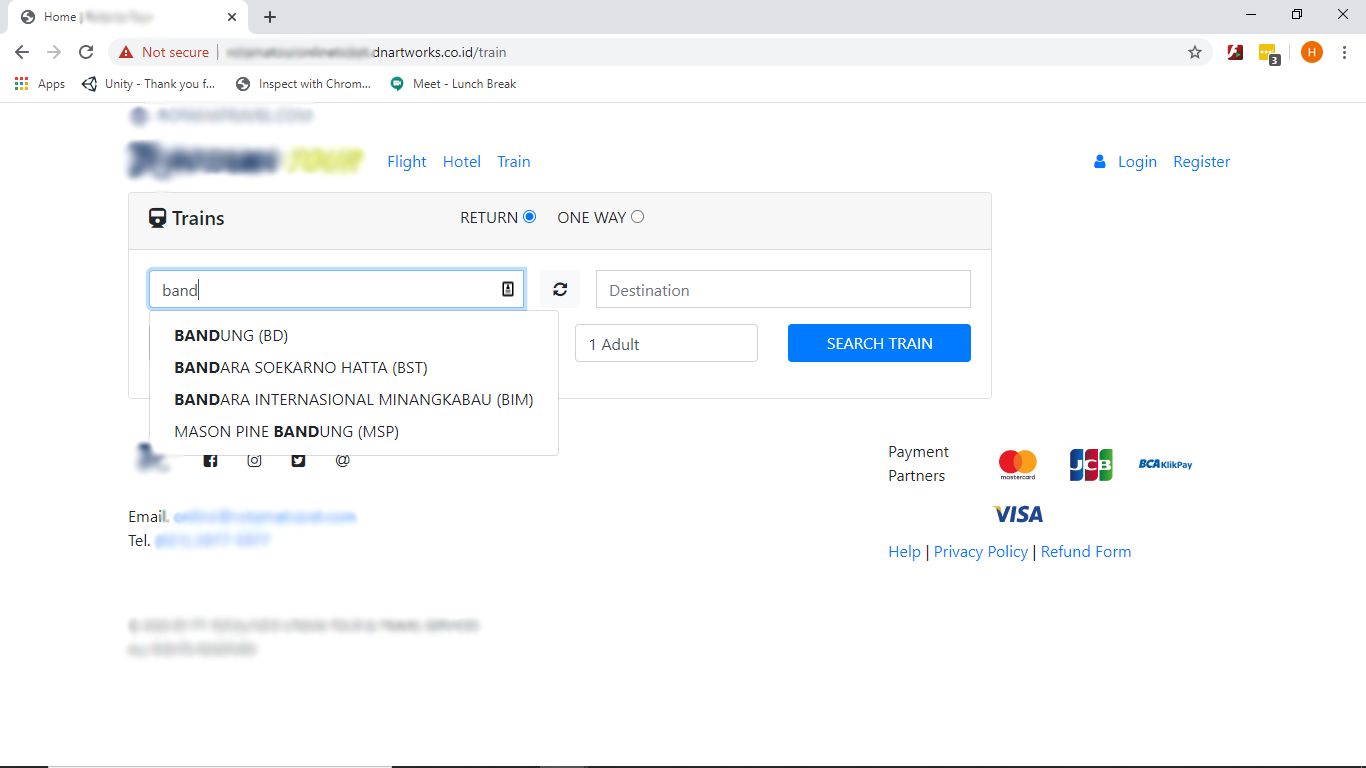
\includegraphics[width=\textwidth,height=\textheight,keepaspectratio]{Gambar/Auto-complete Origin Halaman Pencarian Tiket.png}
        \caption{\textit{Auto-complete} Stasiun Keberangkatan Halaman Pencarian Tiket.}
            \label{img:autocompletestasiunasalcaritiket}
        \end{figure}
        
        Fitur ini berjalan sesuai dengan yang diharapkan seperti dapat dilihat pada gambar \ref{img:autocompletestasiunasalcaritiket} dan \ref{img:autocompletestasiuntujuancaritiket}. Di gambar \ref{img:autocompletestasiunasalcaritiket}, \textit{auto-complete} muncul dari saat pengguna baru memasukkan sebagian dari nama stasiun. Hal yang sama untuk kode dapat dilihat di gambar \ref{img:autocompletestasiuntujuancaritiket}.
        
        \begin{figure}[H]
        \center
        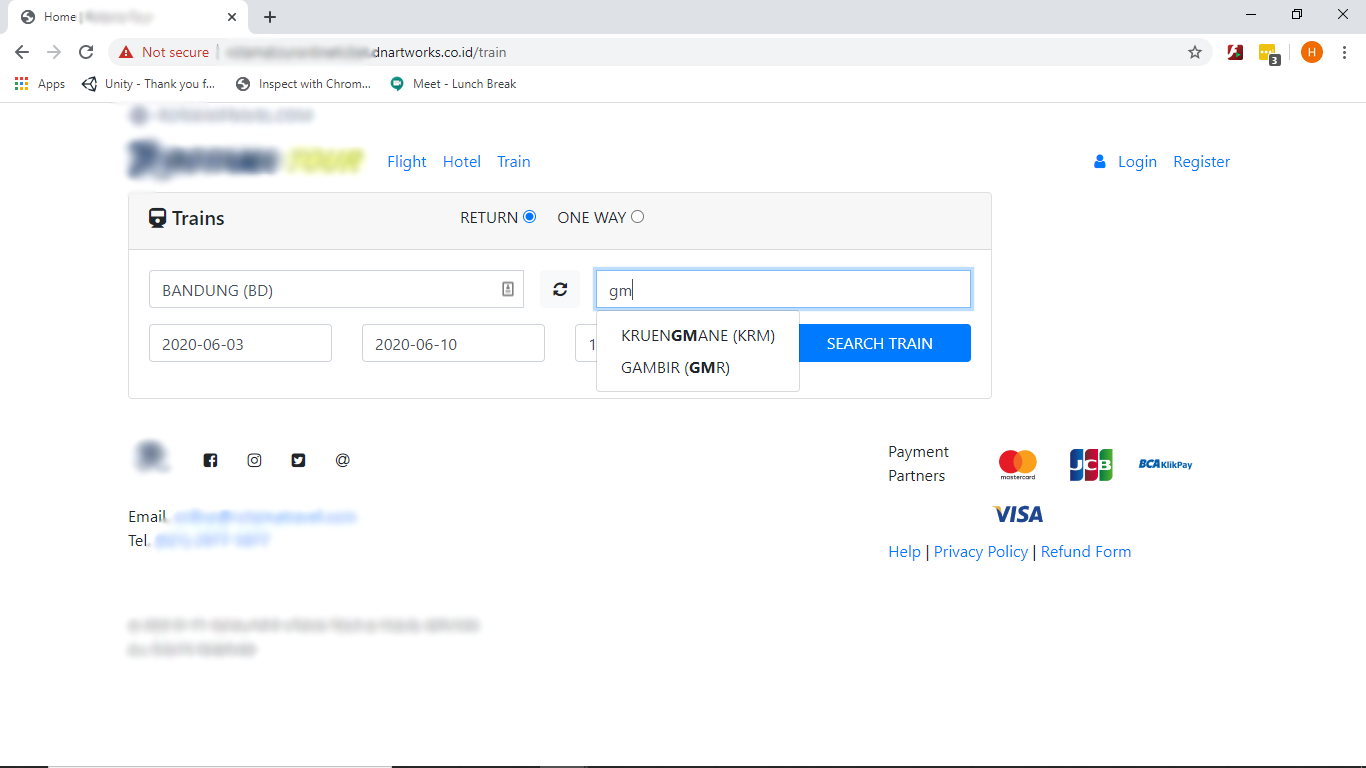
\includegraphics[width=\textwidth,height=\textheight,keepaspectratio]{Gambar/Auto-complete Destination Halaman Pencarian Tiket.png}
        \caption{\textit{Auto-complete} Stasiun Tujuan Halaman Pencarian Tiket.}
            \label{img:autocompletestasiuntujuancaritiket}
        \end{figure}
        
        \item Menguji fungsi \textit{date-picker}.
        
        Tujuan dari pengujian \textit{date-picker} adalah memastikan pengguna tidak bisa memilih tanggal yang tidak \textit{valid}. Tanggal tidak \textit{valid} yang dimaksud adalah tanggal sebelum tanggal hari itu atau tanggal pulang sebelum tanggal keberangkatan. Hal ini ditujukan selain meminimalisir kemungkinan hasil yang kosong, agar tidak terjadi masukan aneh-aneh dari pengguna.
        
        
        \begin{figure}[H]
        \center
        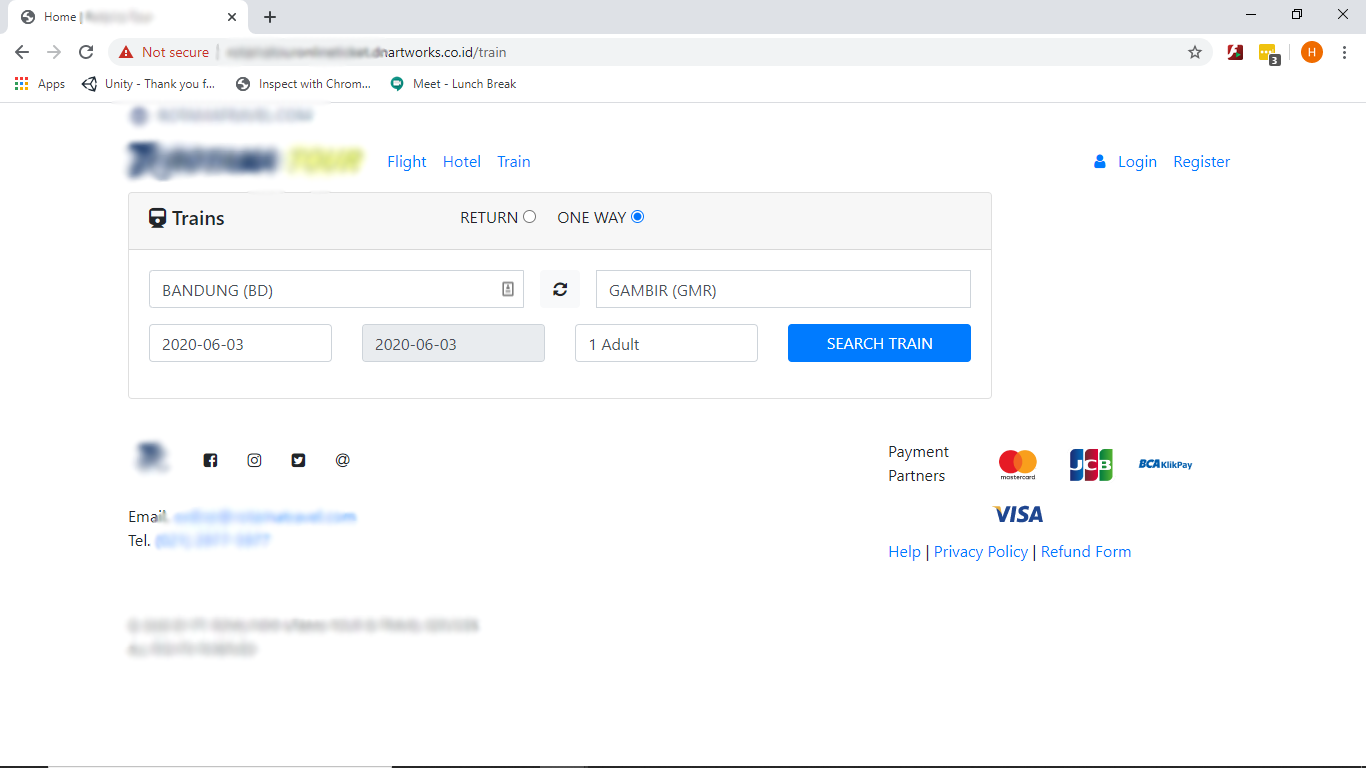
\includegraphics[width=\textwidth,height=\textheight,keepaspectratio]{Gambar/Date-picker one way cari tiket.png}
        \caption{\textit{Date-Picker} Tanggal Pulang saat Perjalanan 1 Arah Halaman Pencarian Tiket.}
            \label{img:datepicker1arah}
        \end{figure}
        
        Dari hasil pengujian, \textit{date-picker} berjalan dengan baik. Dapat dilihat pada gambar \ref{img:datepicker1arah} bahwa pengguna tidak bisa memilih tanggal pulang jika pengguna memilih perjalanan 1 arah. Dari gambar \ref{img:datepickerberangkatcari}, pengguna tidak bisa memilih tanggal sebelum hari itu. Jika pengguna memilih perjalanan 2 arah, pengguna tidak bisa memilih tanggal sebelum tanggal berangkat seperti pada gambar \ref{img:datepickerpulangcari}.
        
        \begin{figure}[H]
        \center
        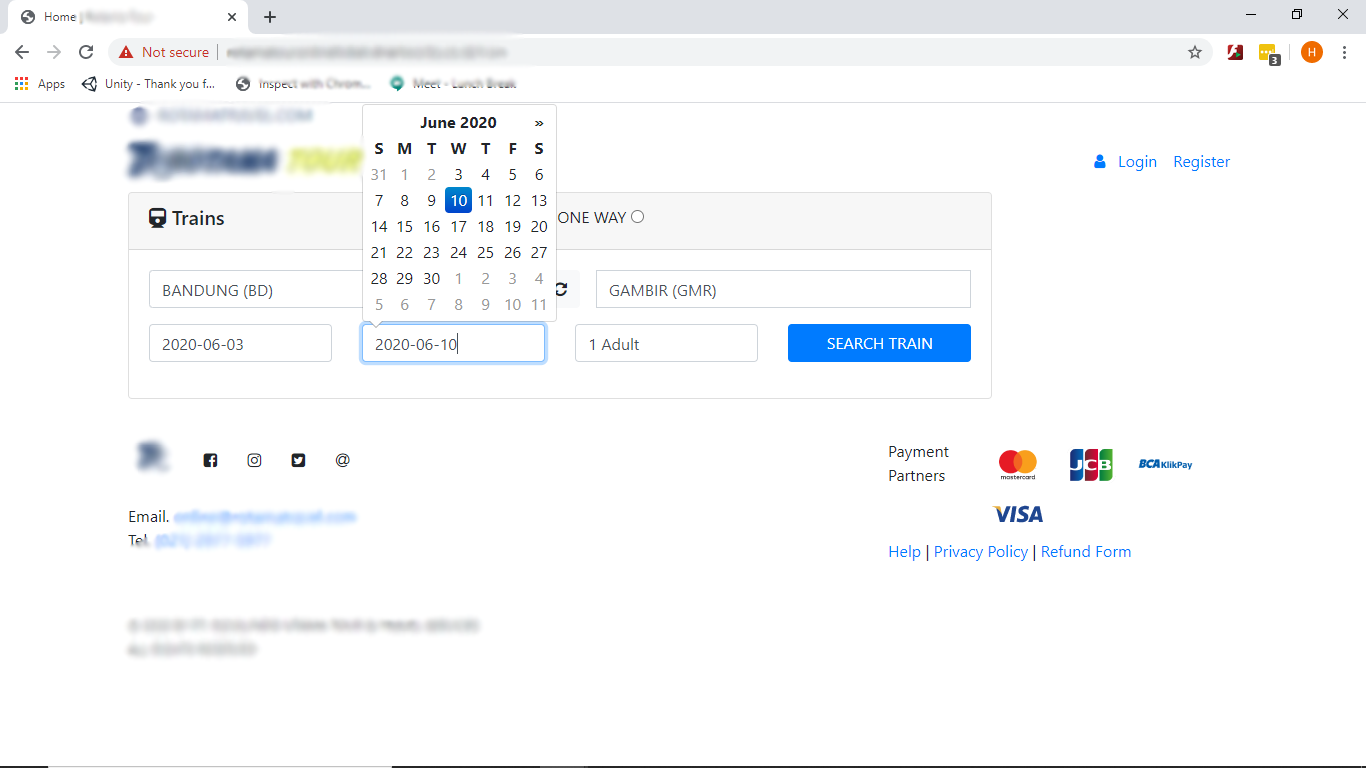
\includegraphics[width=\textwidth,height=\textheight,keepaspectratio]{Gambar/Date-picker tanggal berangkat cari tiket.png}
        \caption{\textit{Date-Picker} Tanggal Berangkat Halaman Pencarian Tiket.}
            \label{img:datepickerberangkatcari}
        \end{figure}
        
        \begin{figure}[H]
        \center
        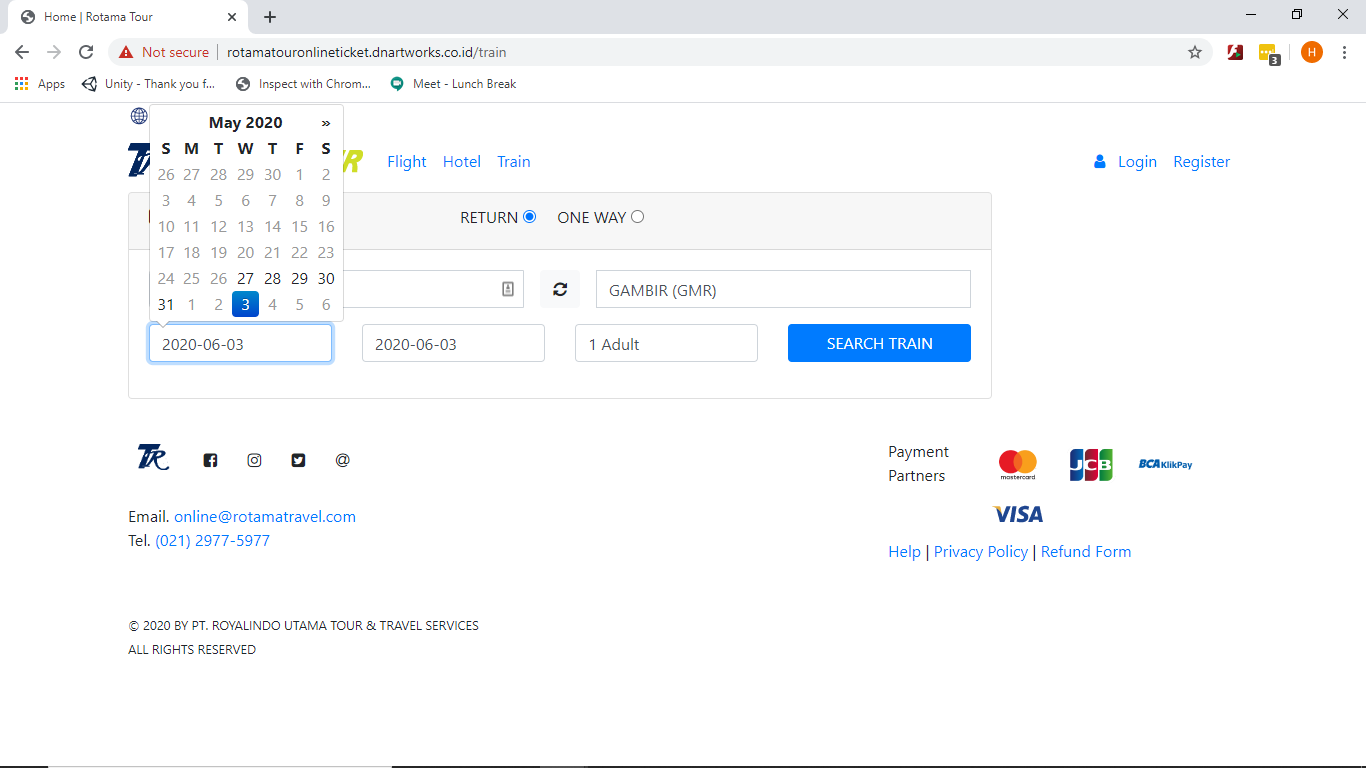
\includegraphics[width=\textwidth,height=\textheight,keepaspectratio]{Gambar/Date-picker tanggal pulang cari tiket.png}
        \caption{\textit{Date-Picker} Tanggal Pulang Halaman Pencarian Tiket.}
            \label{img:datepickerpulangcari}
        \end{figure}
        
        \item Menguji fungsi jumlah penumpang.
        
        Tujuan pengujian fungsi jumlah penumpang adalah mencegah pembelian jumlah tiket yang menyalahi aturan kereta api. Jumlah maksimal penumpang untuk tiap pemesanan adalah 4 penumpang termasuk bayi. Jumlah bayi tidak bisa melebihi jumlah dewasa.
        
        Berdasarkan hasil pengujian, bagian jumlah penumpang berjalan dengan baik. Saat penumpang sudah berjumlah 4, tombol + tidak memberikan efek apapun. Jumlah bayi mengikuti jumlah dewasa sesuai aturan secara otomatis saat jumlah dewasa bertambah atau berkurang.
        
        
        \item Menguji fungsi tombol \textit{search train}.
        
        Tujuan pengujian tombol pencarian ini adalah mengetes apakah pengguna diarahkan dengan benar ke halaman selanjutnya. Tombol ini juga tidak akan mengarahkan pengguna ke halaman selanjutnya jika data belum terisi. Selain itu, saat tombol ini ditekan, proses pencarian jadwal berjalan. Jika terjadi kesalahan pada pemanfaatan \textit{API}, maka tombol ini akan mengarahkan pengguna ke halaman pertama.
        
        \begin{figure}[H]
        \center
        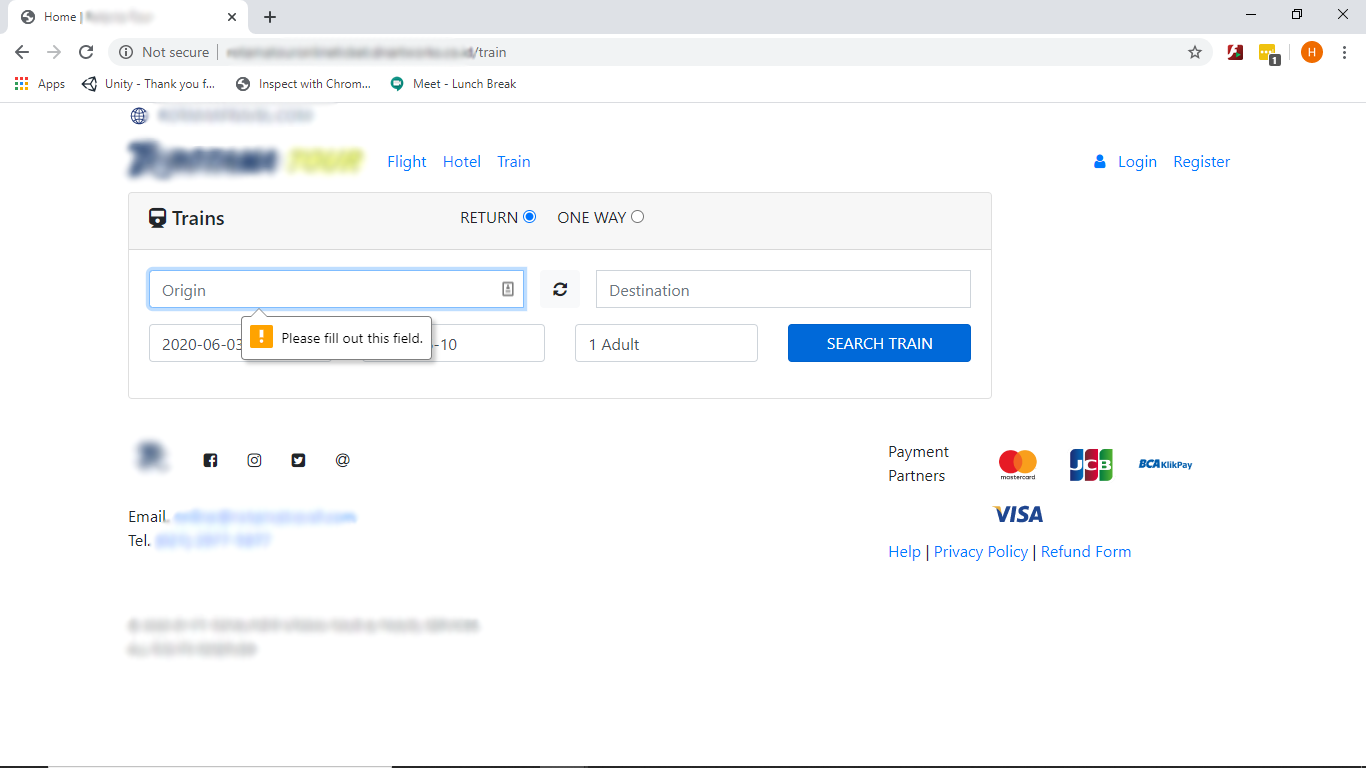
\includegraphics[width=\textwidth,height=\textheight,keepaspectratio]{Gambar/Search train no data pencarian tiket.png}
        \caption{\textit{Search Train} dengan Data yang Belum Terisi Halaman Pencarian Tiket.}
            \label{img:searchnodatacari}
        \end{figure}
        
        Berdasarkan hasil pengujian, karena halaman berhasil diarahkan ke halaman selanjutnya, tombol berjalan dengan baik. \textit{API} diimplementasikan dengan tepat sehingga pengguna tidak diarahkan ke halaman utama kembali. Dapat dilihat peringatan yang diberikan jika pengguna belum mengisi data dengan benar di gambar \ref{img:searchnodatacari}.
        
    \end{enumerate}
    
\subsection{Pengujian Halaman Pemilihan Jadwal.}
\label{subsec:pengujianpilihjadwal}

Hal yang diuji di sini adalah:
    \begin{enumerate}
        \item Menguji ketepatan data yang ditampilkan.
        
        Tujuan pengujian ketepatan data yang ditampilkan adalah memeriksa apakah data yang diminta muncul saat berganti halaman. Selain memunculkan hasil, apakah hasil data yang muncul sesuai dengan permintaan. Terakhir, apakah data yang muncul sudah benar dikelompokkan berdasarkan jadwal berangkat dan pulang.
        
        \begin{figure}[H]
        \center
        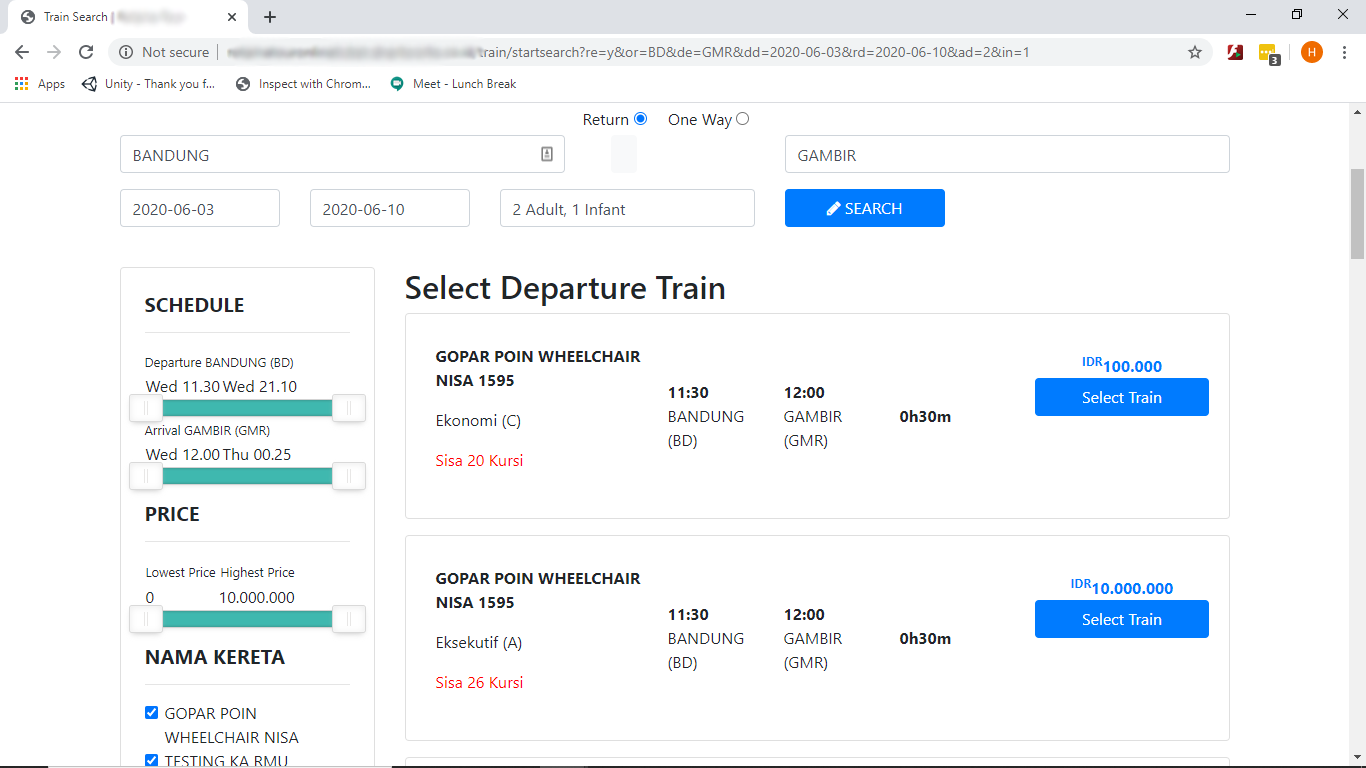
\includegraphics[width=\textwidth,height=\textheight,keepaspectratio]{Gambar/Search result pilih jadwal berangkat.png}
        \caption{Jadwal Berangkat dengan Data yang Diberikan di Halaman Pencarian Tiket.}
            \label{img:searchresultberangkat}
        \end{figure}
        
        \begin{figure}[H]
        \center
        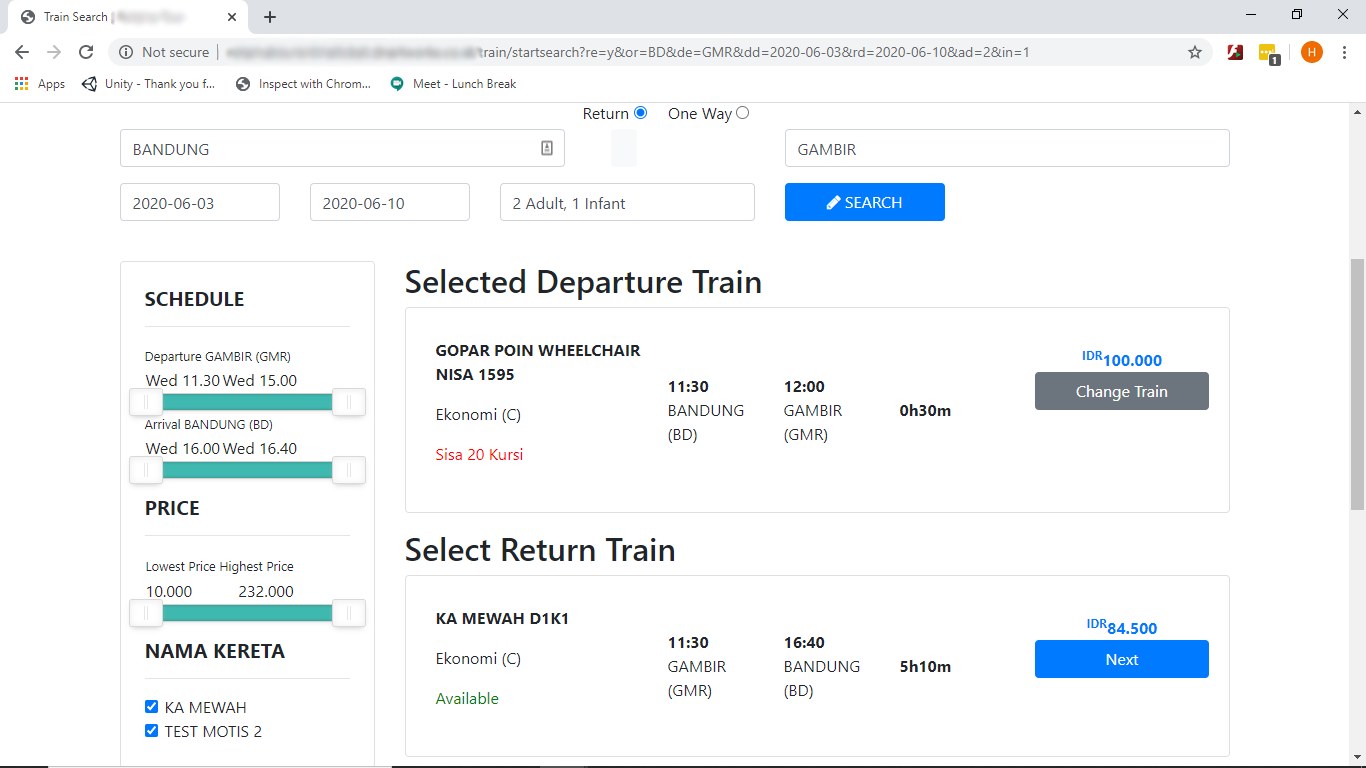
\includegraphics[width=\textwidth,height=\textheight,keepaspectratio]{Gambar/Search result pilih jadwal pulang.png}
        \caption{Jadwal Pulang dengan Data yang Diberikan di Halaman Pencarian Tiket.}
            \label{img:searchresultpulang}
        \end{figure}
        
        Hasil data yang ditunjukkan sesuai dengan permintaan pengguna. Karena masukan pencarian pengguna dibawa juga ke halaman ini di bagian fitur pencarian, maka pengecekan kesesuaian data dapat dilihat langsung di halaman pemilihan jadwal. Hasil jadwal yang ditampilkan pun berhasil dikelompokkan dan dapat dilihat di gambar \ref{img:searchresultberangkat} untuk keberangkatan dan gambar \ref{img:searchresultpulang} untuk pulang. Dapat dilihat juga data yang ditampilkan oleh filter berubah-ubah sesuai dengan jadwal yang ditampilkan.
        
        \item Menguji fungsi halaman pencarian tiket.
        
        Tujuan pengujian 3 fitur pencarian tiket seperti dibahas di \ref{subsec:pengujiancaritiket} adalah agar pengguna tidak usah kembali ke halaman pertama jika ingin melakukan pencarian ulang. Pengguna mungkin salah memasukkan data atau hasil pencarian pengguna tidak sesuai dengan yang diinginkan. Karena adanya 2 kemungkinan itu, maka fitur ini disediakan juga di halaman pencarian tiket.
        
        Ketiga fitur dari halaman sebelumnya berjalan seperti seharusnya di halaman pencarian tiket ini. Perbedaan mendasar yang menjadi kekhawatiran terjadinya kesalahan di sini adalah penambahan data yang sebelumnya sudah diberikan di halaman sebelumnya. Pada versi-versi sebelumnya, data yang dimasukkan dari halaman sebelumnya menghasilkan kesalahan pada fitur tanggal.
        
        \item Menguji filter waktu.
        
        Tujuan pengujian fitur filter berdasarkan waktu adalah agar pengguna bisa lebih mudah memilih waktu yang nyaman bagi dia saat memilih tiket. Pengguna tidak usah melihat satu-satu waktu dari masing-masing jadwal yang tersedia. Hal ini lebih baik digunakan dengan filter karena jika dilakukan dengan \textit{sorting} maka akan timbul pertanyaan mengenai basis pengurutannya. Basis pengurutan yang dimaksud adalah apakah diurutkan berdasarkan waktu berangkat atau waktu tiba.
        
        \begin{figure}[H]
        \center
        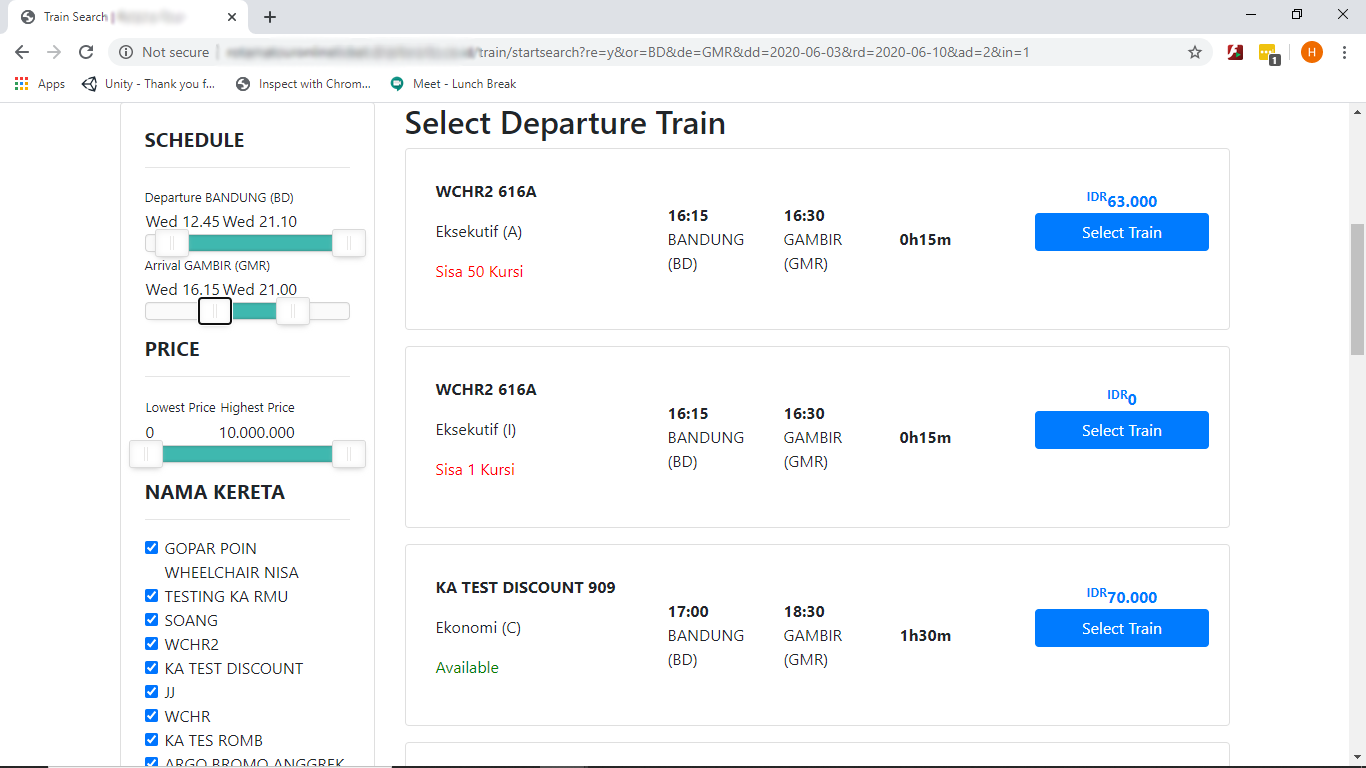
\includegraphics[width=\textwidth,height=\textheight,keepaspectratio]{Gambar/Filter time result.png}
        \caption{Hasil Filter Berdasarkan Waktu untuk Jadwal Berangkat.}
            \label{img:timefilterresult}
        \end{figure}
        
        Dapat dilihat dari gambar \ref{img:timefilterresult} bahwa filter berdasarkan waktu berjalan dengan semestinya. Jika dibandingkan dengan gambar \ref{img:searchresultberangkat}, maka jadwal yang tidak termasuk di \textit{slider} filter waktu, tidak muncul lagi. Hal ini menujukkan filter berhasil dilakukan.
        
        \item Menguji filter harga.
        
        Tujuan filter berdasarkan harga adalah untuk membantu pengguna menemukan jadwal yang sesuai dengan budget. Filter harga menyembunyikan hasil jadwal yang di luar jangkauan pengguna. Filter dipilih di sini karena jika menggunakan \textit{sorting}, ada kemungkinan hasil yang didapat banyak dan pengguna akan habis waktu mencari satu per satu ke jarak harga yang pengguna mau.
        
        \begin{figure}[H]
        \center
        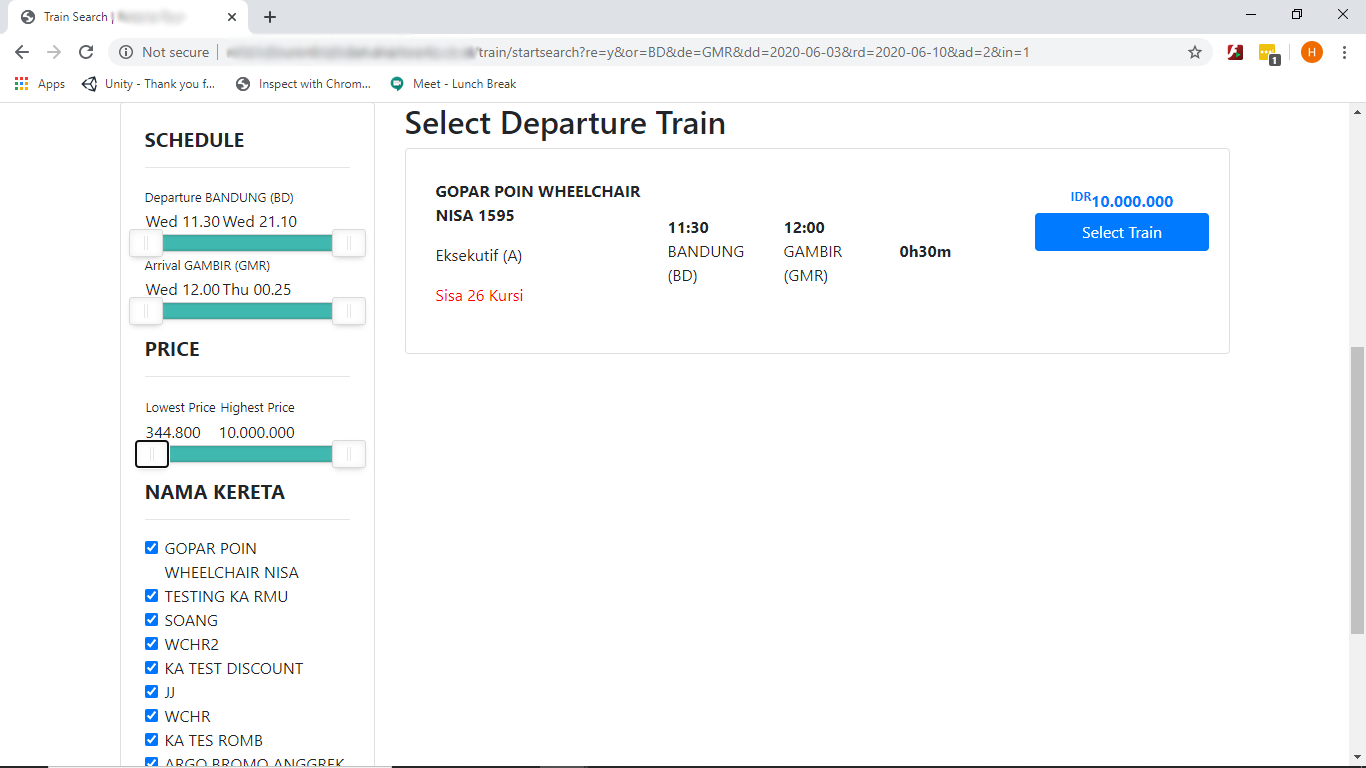
\includegraphics[width=\textwidth,height=\textheight,keepaspectratio]{Gambar/Filter price result.png}
        \caption{Hasil Filter Berdasarkan Harga untuk Jadwal Berangkat.}
            \label{img:pricefilterresult}
        \end{figure}
        
        Berdasarkan gambar \ref{img:pricefilterresult}, filter berdasarkan harga berjalan dengan seharusnya. Jika dibandingkan dengan gambar \ref{img:searchresultberangkat}, maka jadwal yang di luar jangkauan harga di \textit{slider} filter harga, tidak muncul. Hal ini menujukkan filter berhasil dilakukan.
        
        \item Menguji filter nama kereta.
        
        Tujuan pengujian fitur filter berdasarkan nama kereta adalah agar pengguna bisa lebih mudah memilih jasa kereta yang pengguna sudah kenal. Filter dilakukan menggunakan \textit{checkbox} agar pengguna dengan mudah menghilangkan pilihan yang pengguna tidak inginkan. Dengan menggunakan \textit{checkbox}, pengguna bisa menyisakan beberapa nama kereta yang pengguna kenal dan memilih jadwal mana yang pengguna inginkan.
        
        \begin{figure}[H]
        \center
        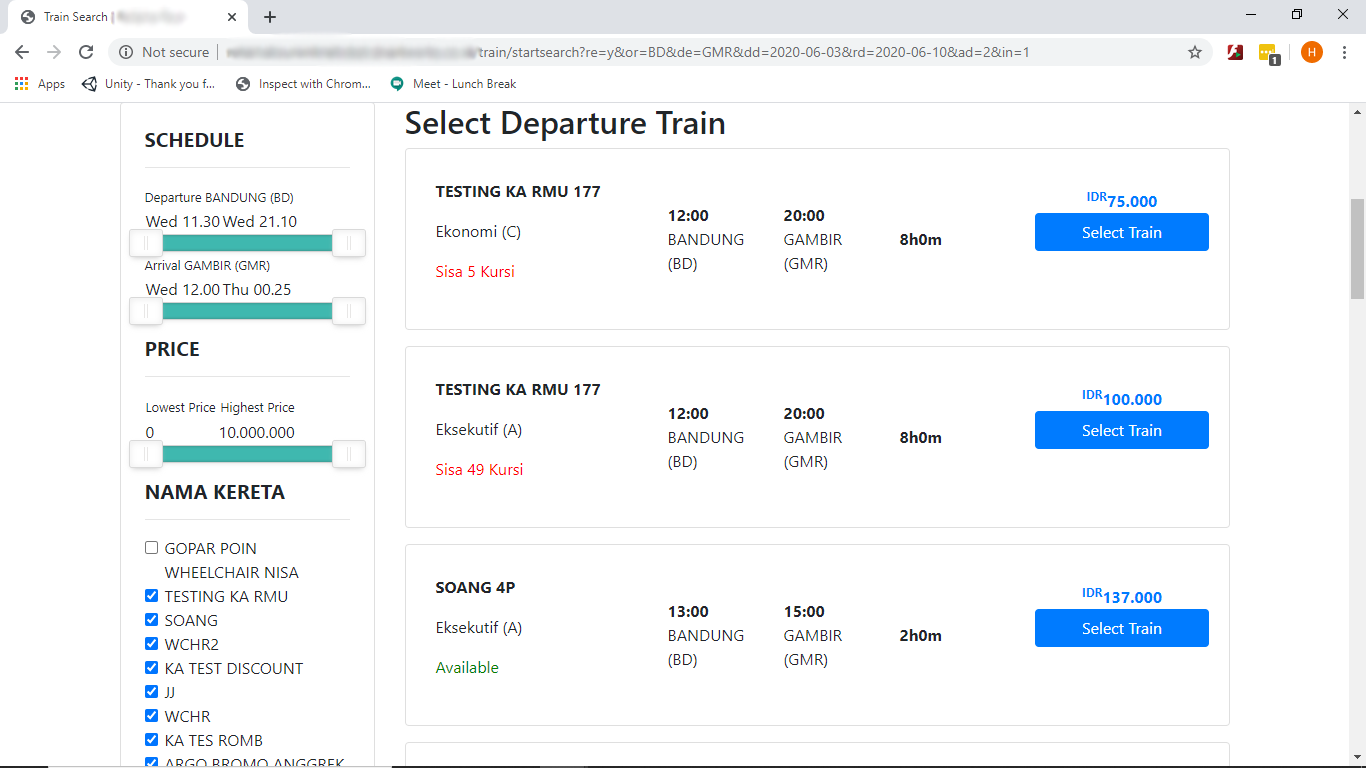
\includegraphics[width=\textwidth,height=\textheight,keepaspectratio]{Gambar/Filter name result.png}
        \caption{Hasil Filter Berdasarkan Nama untuk Jadwal Berangkat.}
            \label{img:namefilterresult}
        \end{figure}
        
        Sesuai dengan gambar \ref{img:namefilterresult}, filter berdasarkan nama berjalan dengan baik. Jika dibandingkan dengan gambar \ref{img:searchresultberangkat}, maka jadwal dengan nama yang tidak diceklis tidak akan ditampilkan. Dalam kasus ini, jadwal harusnya ada di paling atas hilang karena nama keretanya tidak diceklis yang berarti filter ini berjalan.
        
        \item Menguji tombol \textit{select train}.
        
        Pengujian tombol \textit{select train} dilakukan dengan tujuan agar bisa membagi antara jadwal berangkat dan jadwal pulang jika pengguna memilih perjalanan pulang pergi. Saat \textit{select train} ditekan maka tulisan \textit{departure} berubah menjadi \textit{return}. Jadwal berangkat yang dipilih akan ditampilkan di atas jadwal pulang. Tombol ini berfungsi dengan baik dan dapat diamati di \ref{img:searchresultberangkat} dan \ref{img:searchresultpulang}.
        
        \item Menguji tombol \textit{change train}.
        
        Pengujian tombol \textit{change train} juga diperlukan untuk memastikan data yang ditampilkan kembali dari jadwal pulang ke jadwal berangkat. Saat ditekan, tulisan \textit{return} kembali menjadi \textit{departure} dan jadwal yang ditampilkan kembali menjadi jadwal berangkat. Jadwal berangkat yang dipilih sebelumnya akan hilang. Dari hasil pengujian, tombol ini berjalan dengan baik.
        
        \item Menguji tombol \textit{next}.
        
        Tujuan tombol \textit{next} adalah menampilkan \textit{pop-up} yang berisi data yang dipilih. \textit{Pop-up} yang muncul adalah \textit{pop-up} konfirmasi agar pengguna bisa memastikan pilihannya sudah benar. Saat tombol ditekan, \textit{pop-up} muncul tanpa masalah seperti dapat dilihat pada gambar \ref{img:popuppilihjadwal}.
        
        \begin{figure}[H]
        \center
        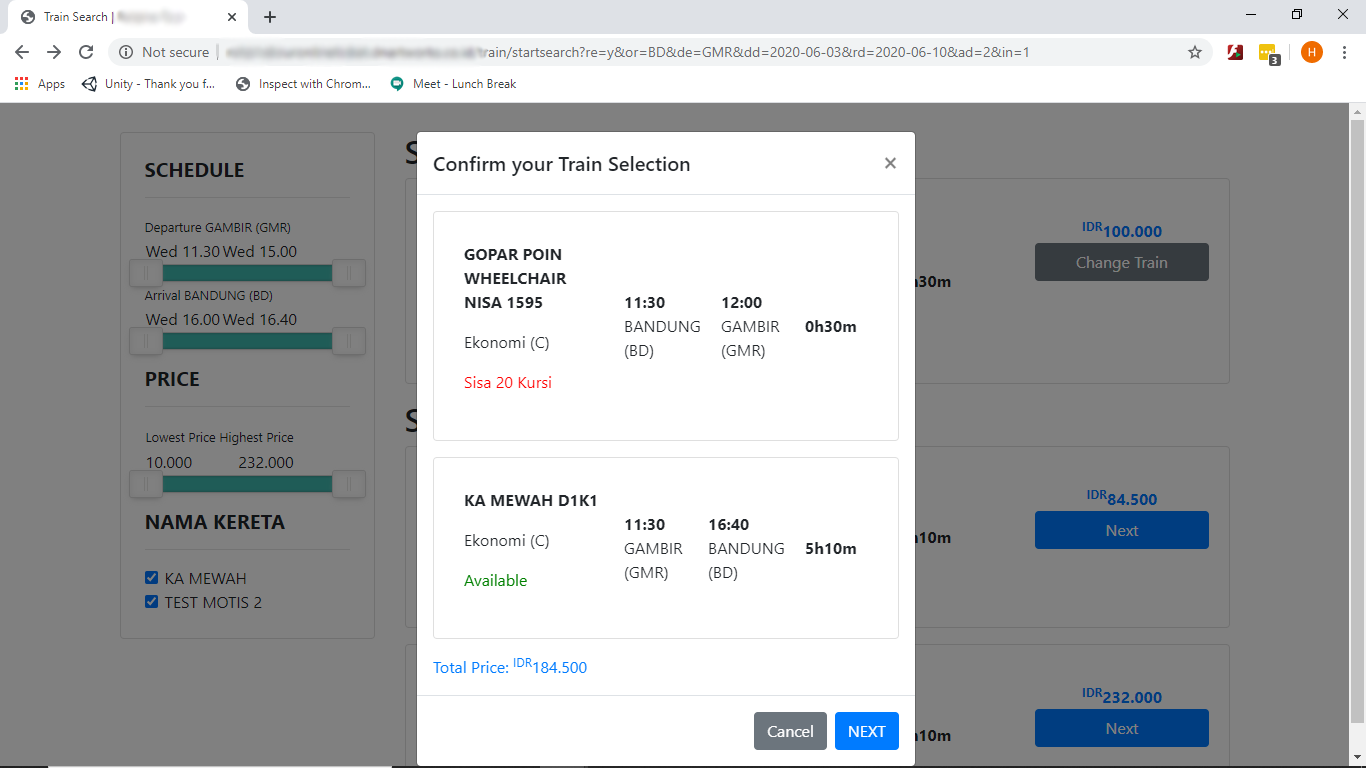
\includegraphics[width=\textwidth,height=\textheight,keepaspectratio]{Gambar/Konfirmasi pilih jadwal.png}
        \caption{\textit{Pop-up} Konfirmasi untuk Halaman Pemilihan Jadwal.}
            \label{img:popuppilihjadwal}
        \end{figure}
        
        \item Menguji tombol \textit{close} dan \textit{cancel}.
        
        Tombol \textit{close} dan \textit{cancel} digunakan jika pengguna ingin mengganti pilihannya setelah \textit{pop-up} muncul. Tombol ini tidak mengembalikan halaman seperti semula (\textit{refresh}) saat ditekan. Saat salah satu tombol ditekan atau saat pengguna menekan di luar \textit{pop-up}, \textit{pop-up} tertutup yang berarti tombol ini berjalan sesuai dengan harapan.
        
        \item Menguji tombol \textit{next} \textit{pop-up}.
        
        Tombol \textit{next} untuk \textit{pop-up} adalah tombol yang mengarahkan pengguna ke halaman pengisian data. Saat pengguna sudah yakin dengan pilihannya, pengguna akan menekan tombol ini. Tombol ini berhasil mengarahkan pengguna ke halaman selanjutnya yang berarti data yang diberikan ke halaman selanjutnya sudah tepat dan tombol ini berfungsi sesuai ekspektasi.
        
    \end{enumerate}
    
\subsection{Pengujian Halaman Pengisian Data Penumpang.}
\label{subsec:pengujianisidata}

Hal yang diuji di sini adalah:
    \begin{enumerate}
        \item Menguji ketepatan data yang ditampilkan.
        
        Pengujian ini memastikan data yang ditampilkan di halaman pengisian data penumpang sesuai dengan halaman sebelumnya. Dapat dilihat dari gambar \ref{img:sidebarisidata1} dan \ref{img:sidebarisidata2} dengan membandingkan dengan gambar \ref{img:searchresultberangkat} dan \ref{img:popuppilihjadwal} bahwa data sudah sesuai. Data kereta dan harga sesuai dengan \textit{pop-up} dari \ref{subsec:pengujianpilihjadwal} sementara jumlah penumpang dan jenisnya sama dengan masukan pencarian.
        
        \begin{figure}[H]
        \center
        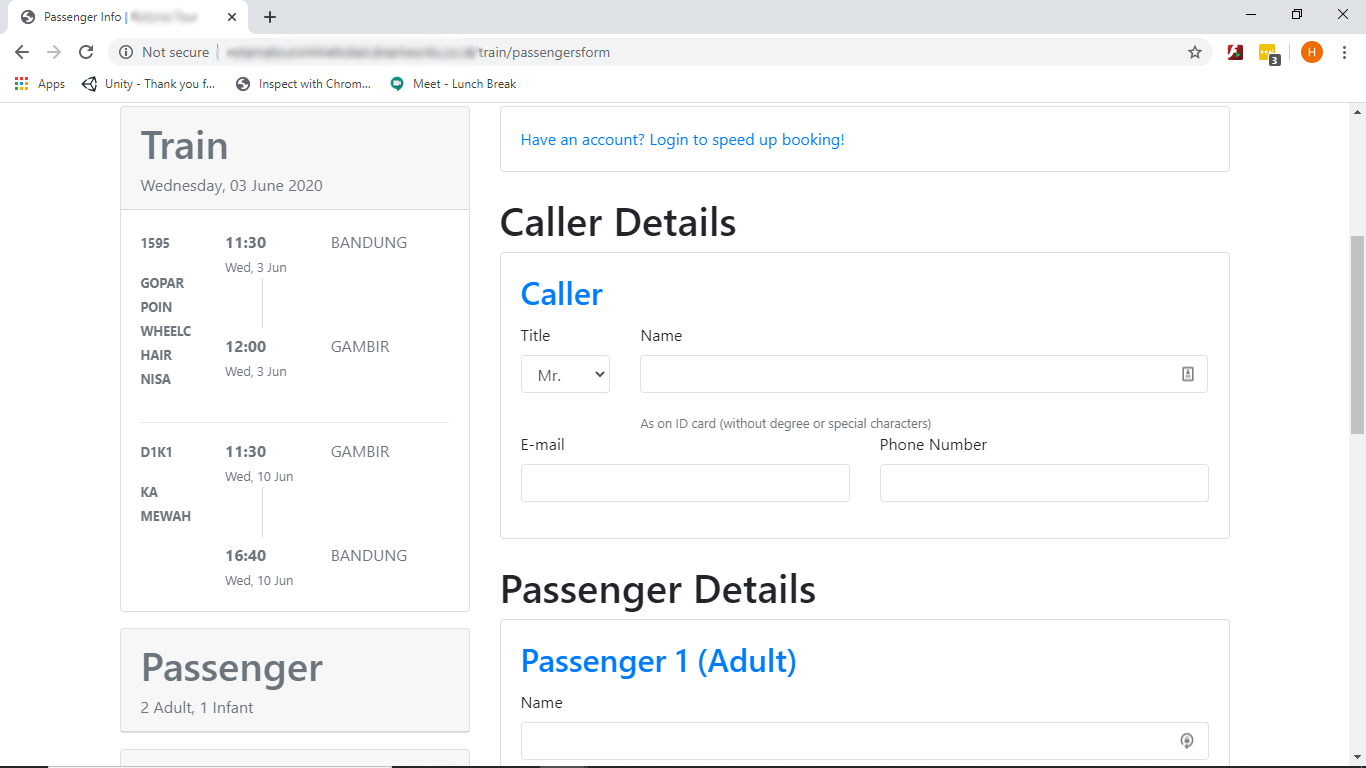
\includegraphics[width=\textwidth,height=\textheight,keepaspectratio]{Gambar/Sidebar isi data 1.png}
        \caption{Sidebar Pengisian Data 1.}
            \label{img:sidebarisidata1}
        \end{figure}
        
        \begin{figure}[H]
        \center
        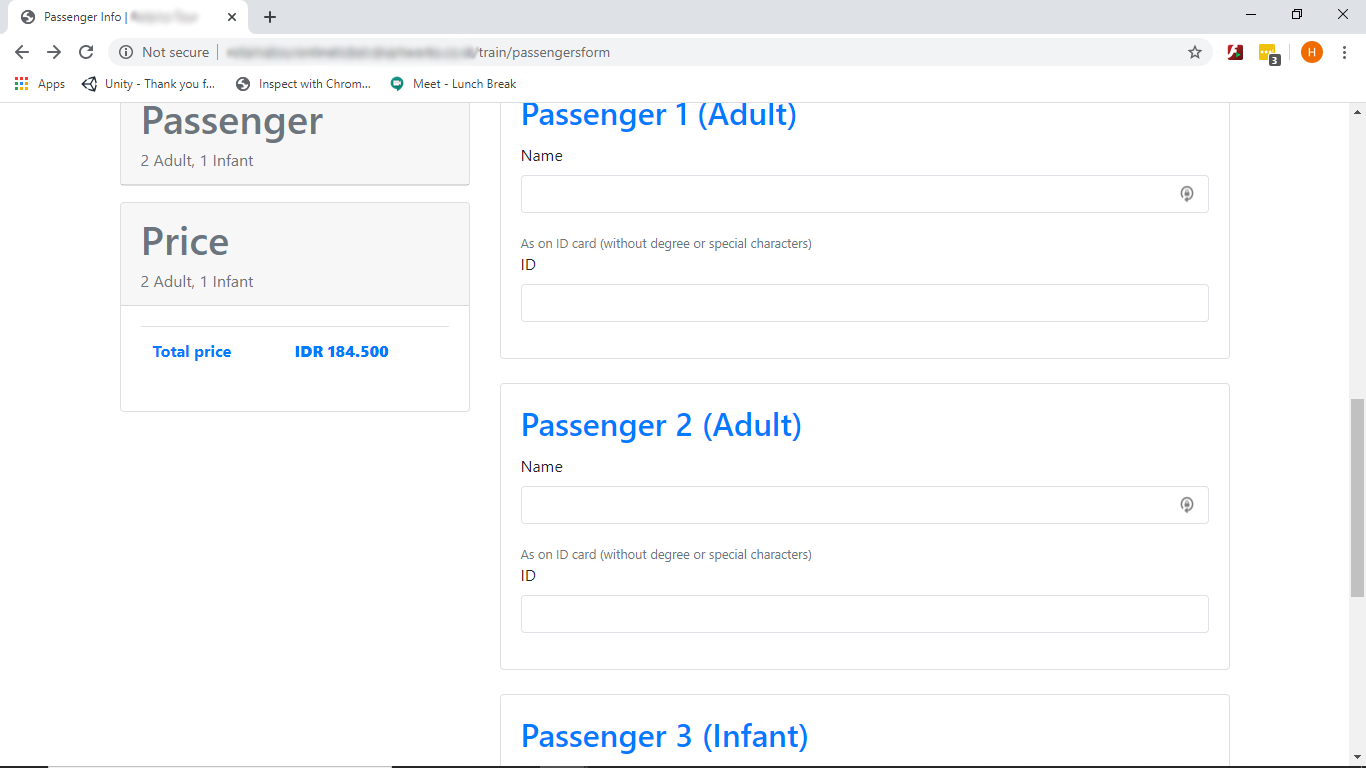
\includegraphics[width=\textwidth,height=\textheight,keepaspectratio]{Gambar/Sidebar isi data 2.png}
        \caption{Sidebar Pengisian Data 2.}
            \label{img:sidebarisidata2}
        \end{figure}
        
        \item Menguji fitur \textit{login}.
        
        Fitur \textit{login} digunakan untuk mempercepat proses pengisian data. Pengguna dapat mengakses fitur \textit{fill from address book} jika pengguna sudah terdaftar dan sudah \textit{login}. Fitur ini berjalan dengan lancar karena dengan mengklik tautan \textit{login}, pengguna akan diarahkan ke halaman \textit{login} seperti gambar \ref{img:halamanlogin}.
        
        \begin{figure}[H]
        \center
        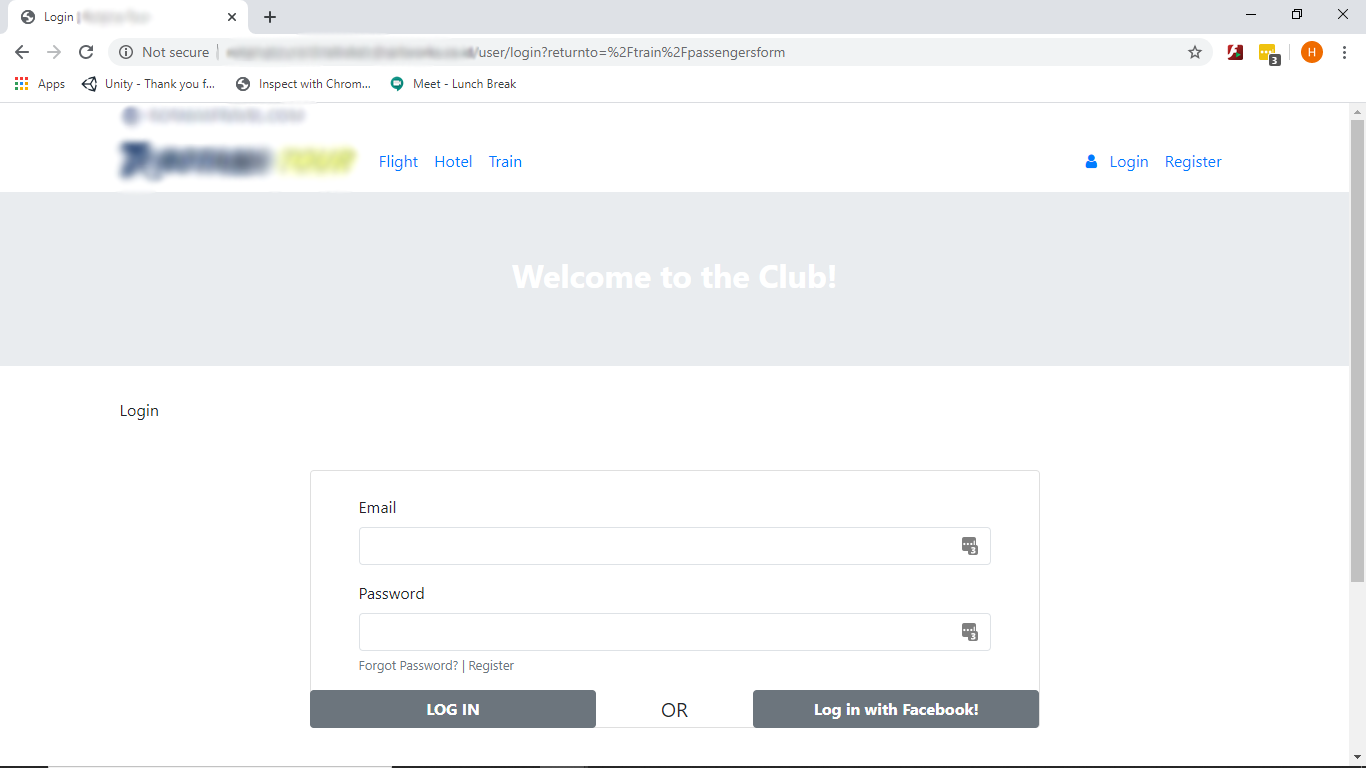
\includegraphics[width=\textwidth,height=\textheight,keepaspectratio]{Gambar/Login screen.png}
        \caption{Halaman \textit{Login}.}
            \label{img:halamanlogin}
        \end{figure}
        
        \item Menguji fitur \textit{auto-fill}.
        
        Fitur \textit{auto-fill} atau fitur \textit{fill from address book} adalah fitur yang membantu pengguna untuk mengisi data lebih cepat jika pengguna sudah \textit{login}. Pengguna bisa memilih data mana yang ingin diisikan pada bagian mana dengan memilih dari \textit{dropbox} seperti pada gambar \ref{img:filladdressbook}. Fitur ini akan mengisi data-data yang diperlukan dengan informasi yang sudah disimpan sebelumnya saat pengguna mendaftar. Fitur ini berjalan dengan baik berdasarkan hasil uji.
        
        \item Menguji tombol \textit{select seat}.
        
        Tombol \textit{select seat} adalah tombol opsional untuk pengguna yang ingin memilih kursi. Tombol ini akan memunculkan \textit{pop-up} saat ditekan. Saat pengguna menekan \textit{next} tapi data belum terisi dengan lengkap maka muncul peringatan  seperti pada gambar \ref{img:nodatanextisidata}. Tombol ini akan mengarahkan pengguna ke halaman pencarian tiket jika pengguna menekan \textit{next} setelah menekan tombol \textit{select seat}. Tombol ini berhasil menampilkan halaman selanjutnya yang dapat dilihat pada \ref{subsec:pengujianpilihkursi} yang berarti tombol berfungsi dengan benar.
        
        \begin{figure}[H]
        \center
        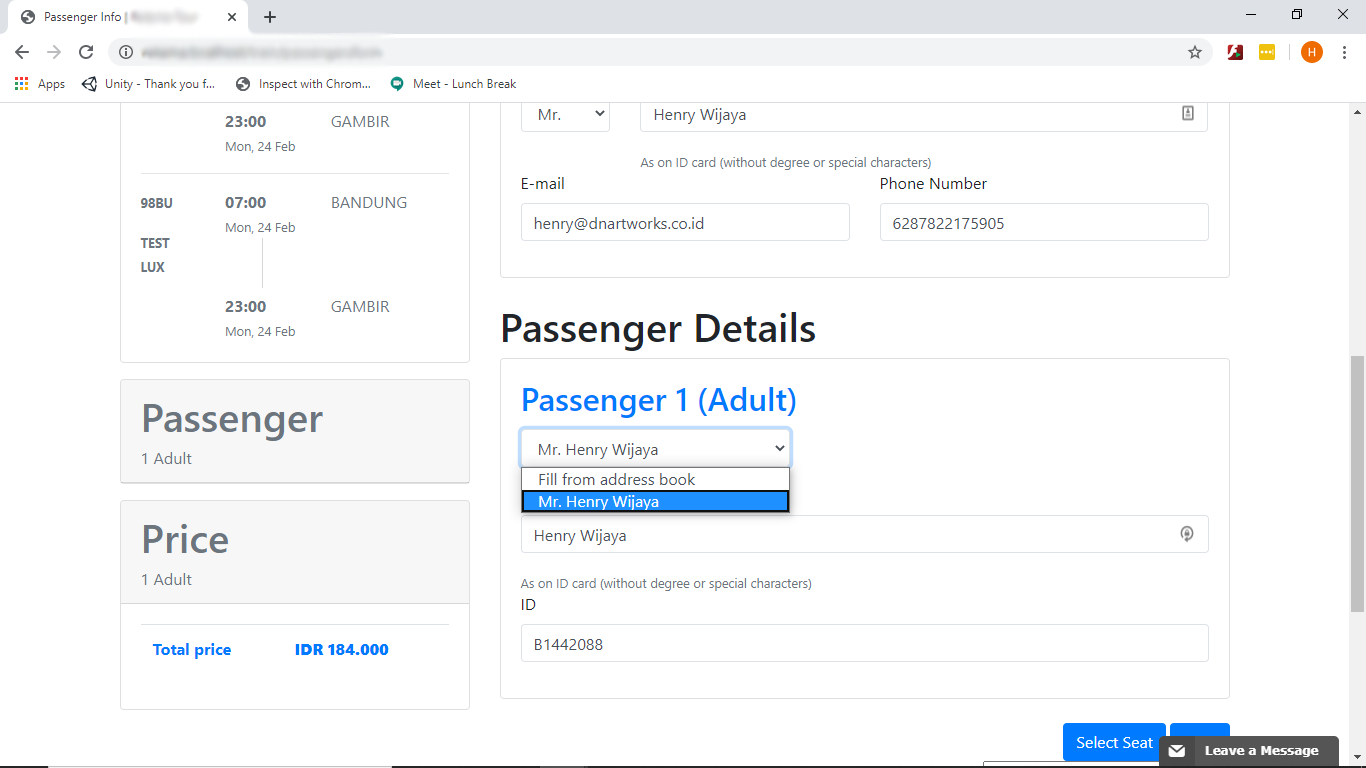
\includegraphics[width=\textwidth,height=\textheight,keepaspectratio]{Gambar/Fill from address book isi data.png}
        \caption{\textit{Dropdown} dan Hasil \textit{Fill from Address Book}.}
            \label{img:filladdressbook}
        \end{figure}
        
        
        
        \begin{figure}[H]
        \center
        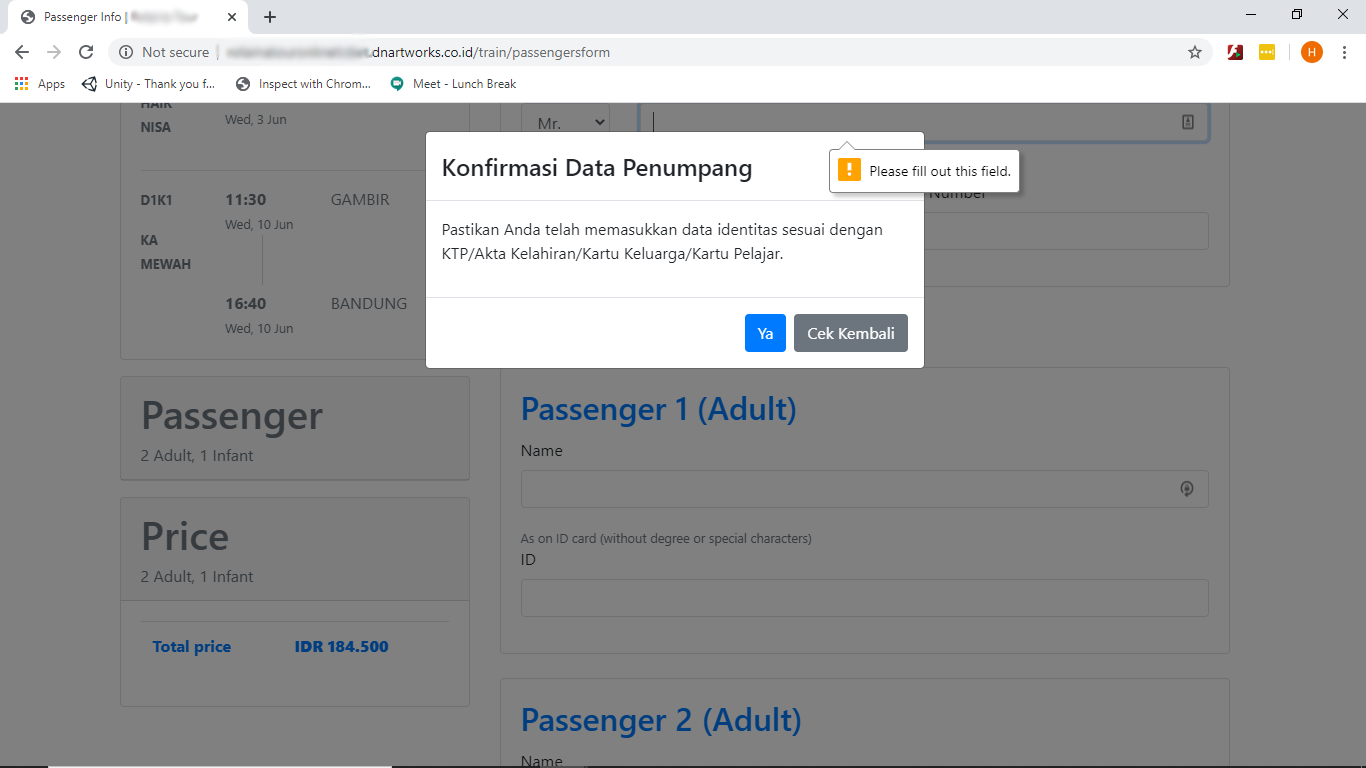
\includegraphics[width=\textwidth,height=\textheight,keepaspectratio]{Gambar/Data belum terisi pengisian data penumpang.png}
        \caption{Data Belum Terisi saat Konfirmasi.}
            \label{img:nodatanextisidata}
        \end{figure}
        
        \item Menguji next \textit{next}.
        
        Tombol \textit{next} ini memiliki fungsi yang sama dengan tombol \textit{select seat}. Perbedaan kedua tombol ini adalah tombol \textit{next} akan mengarahkan pengguna ke halaman konfirmasi jika ditekan. Tombol ini berfungsi dengan baik karena berhasil mengarahkan pengguna ke halaman konfirmasi yang dapat dilihat di \ref{subsec:pengujiankonfirmasi}.
        
    \end{enumerate}
    
\subsection{Pengujian Halaman Pemilihan Tempat Duduk.}
\label{subsec:pengujianpilihkursi}

Hal yang diuji di sini adalah:
    \begin{enumerate}
        \item Menguji ketepatan tampilan.
        
        Tujuan pengujian ini adalah memastikan tampilan data dan pemetaan kursi sesuai dengan data yang ada. Untuk memastikan tampilan kursi benar, maka data hasil keluaran \textit{API} harus dilihat dan dibandingkan. Input yang didapat bisa dilihat di bawah. Tampilan yang dibuat berdasarkan input dapat diformat sesuai dengan kemauan. Untuk kasus ini, baris dan kolom ditukar agar peta kereta panjang menyamping.
        
        \begin{lstlisting}[language=json]
            {
                "err_num": "0",
                "err_str": "OK",
                "result": {
                    "seat_map": [
                        [
                            "LUX",
                            1,
                            [
                                [
                                    1,
                                    3,
                                    1,
                                    "B",
                                    "A",
                                    1
                                ],
                                [
                                    1,
                                    4,
                                    1,
                                    "C",
                                    "A",
                                    ""
                                ],
                                ...
                                 [
                                    11,
                                    4,
                                    11,
                                    "C",
                                    "A",
                                    ""
                                ],
                                [
                                    12,
                                    1,
                                    12,
                                    "A",
                                    "A",
                                    ""
                                ]
                            ]
                        ],
                        ...
        \end{lstlisting}
        
        Dari potongan hasil respon \textit{API} di atas, seperti yang dijelaskan pada \ref{subsec:getrailseatmap}, dapat disimpulkan bahwa kereta memiliki 12 kolom dan 3 baris. Kolom-kolom dinamai dengan angka dari 1-12 dan baris dinamai dari A-C dengan sebuah baris kosong. Baris kosong dapat diketahui karena dari data baris dan kolom, yang diberikan, tidak ada data baris 2 yang berarti baris A ada terpisah dari baris B dan C. Dengan membandingkan kesimpulan yang didapatkan dan gambar \ref{img:seatselection1}, dapat dilihat bahwa pemetaan kereta sudah benar.
        
        \begin{figure}[H]
        \center
        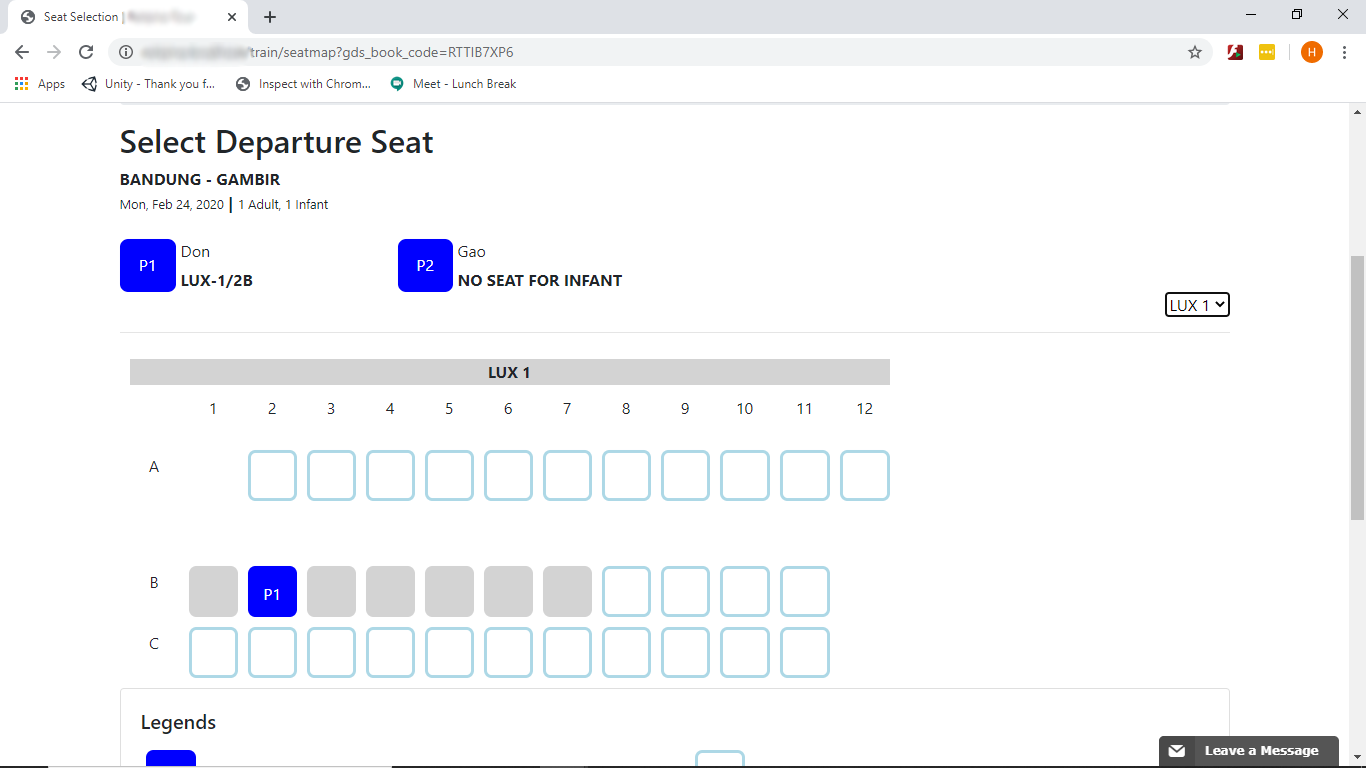
\includegraphics[width=\textwidth,height=\textheight,keepaspectratio]{Gambar/Seat selection 1.png}
        \caption{Halaman Pemilihan Kursi.}
            \label{img:seatselection1}
        \end{figure}
        
        \item Menguji \textit{dropbox} pemilihan kereta.
        
        Tujuan dari \textit{dropbox} pemilihan kereta adalah karena beberapa kereta memiliki beberapa wagon. \textit{Dropbox} ini membantu pengguna untuk memilih wagon berapa yang mereka ingin pilih. \textit{Dropbox} berfungsi dengan baik berdasarkan tampilan wagon 2 di gambar \ref{img:seatselection2}.
        
        \begin{figure}[H]
        \center
        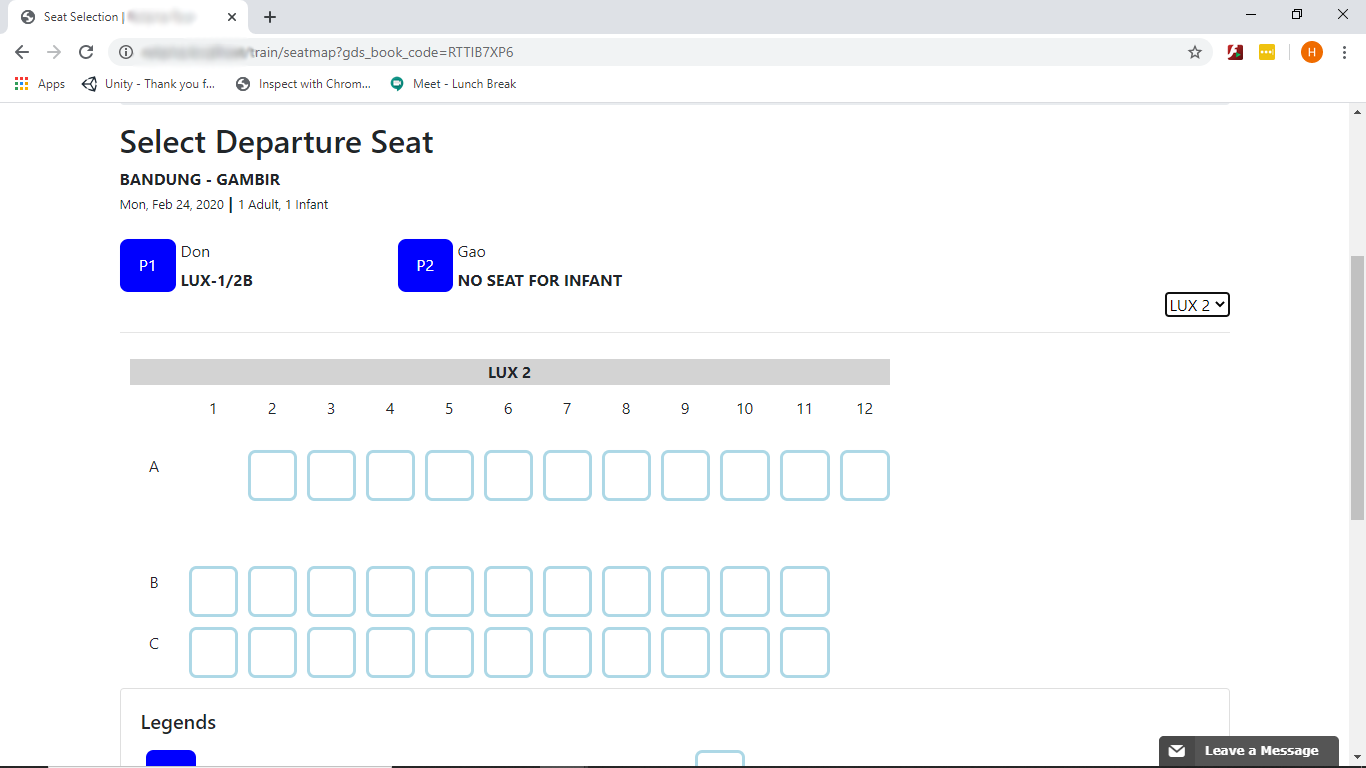
\includegraphics[width=\textwidth,height=\textheight,keepaspectratio]{Gambar/Seat selection 2.png}
        \caption{Menampilkan Wagon 2 sesuai dengan \textit{dropbox}.}
            \label{img:seatselection2}
        \end{figure}
        
        \item Menguji pemilihan tempat duduk.
        
        Memilih tempat duduk dilakukan dengan menekan tempat yang diinginkan sejumlah penumpang dewasa. Tempat pertama yang berhasil ditekan adalah tempat penumpang dewasa pertama dan seterusnya. Berdasarkan aturan KAI, bayi tidak mendapatkan kursi sehingga pemilihan kursi hanya dilakukan sesuai jumlah penumpang dewasa. Berdasarkan gambar \ref{img:pilihtempatduduk}, pemilihan kursi bisa dilakukan dengan lancar. Dapat dilihat juga tempat duduk pengguna di atas peta berbeda dengan tempat duduk awal pengguna yang dapat diamati dari peta.
        
         \item Menguji tombol \textit{restore default}.
        
        Tombol \textit{restore default} adalah tombol yang digunakan untuk mengembalikan pilihan kursi ke kondisi awal. Tombol ini disediakan jika pengguna salah memilih tempat atau berubah pikiran saat sudah memilih. Tombol ini mengembalikan kondisi awal terpisah untuk keberangkatan dan pulang. Pengguna bisa mengembalikan kursi berangkat ke kondisi awal tanpa mengembalikan kursi pulang ke kondisi awal. Setelah diuji, tombol ini berjalan dengan baik.
        
         \item Menguji tombol \textit{next train}.
        
        Tombol \textit{next train} akan mengganti tampilan pilih kursi dari kursi berangkat menjadi kursi pulang. Tombol ini hanya akan muncul jika pengguna memilih perjalanan pulang pergi. Seperti yang bisa diamati dari gambar \ref{img:pilihkursiberangkat} dan \ref{img:pilihkursipulang}, tombol berjalan dengan baik.
        
        \begin{figure}[H]
        \center
        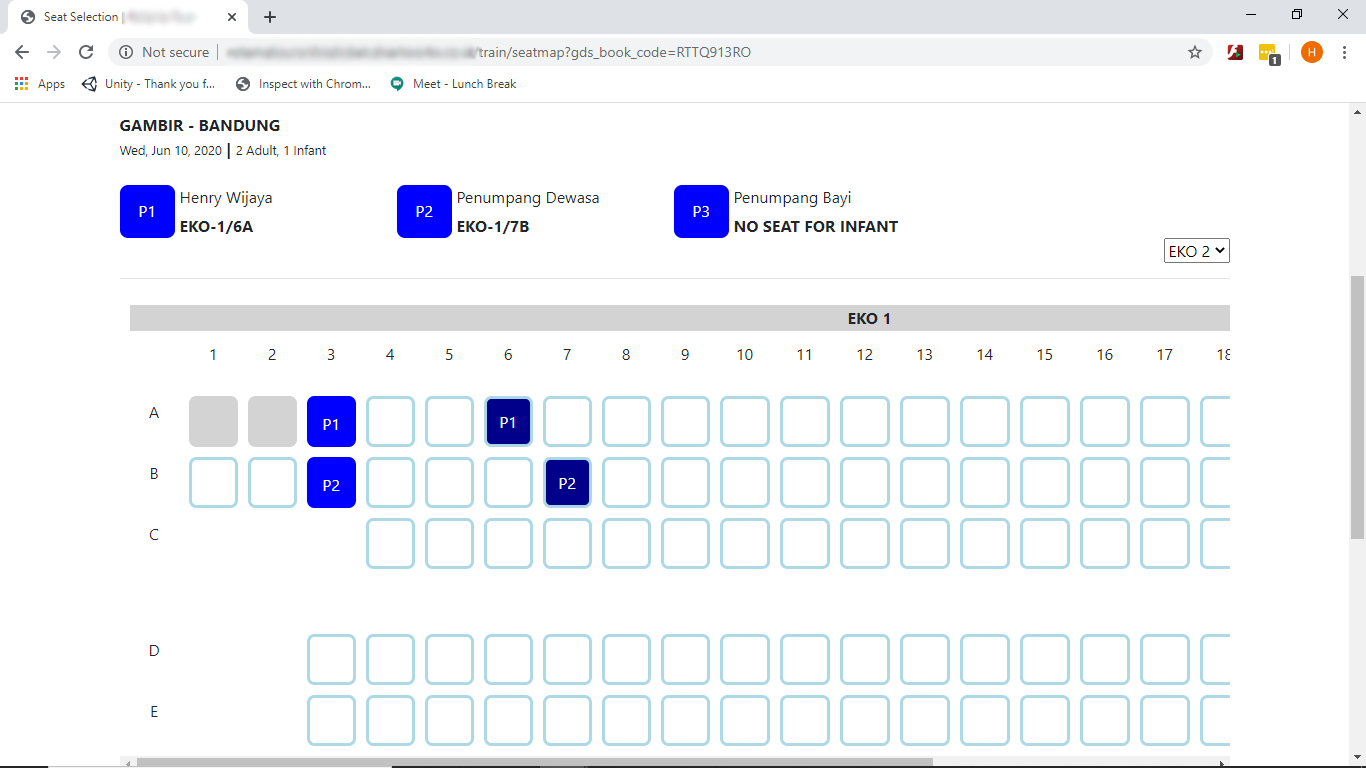
\includegraphics[width=\textwidth,height=\textheight,keepaspectratio]{Gambar/Pilih Tempat Duduk.png}
        \caption{Hasil Pemilihan Tempat Duduk.}
            \label{img:pilihtempatduduk}
        \end{figure}
        
       
    
        
        \begin{figure}[H]
        \center
        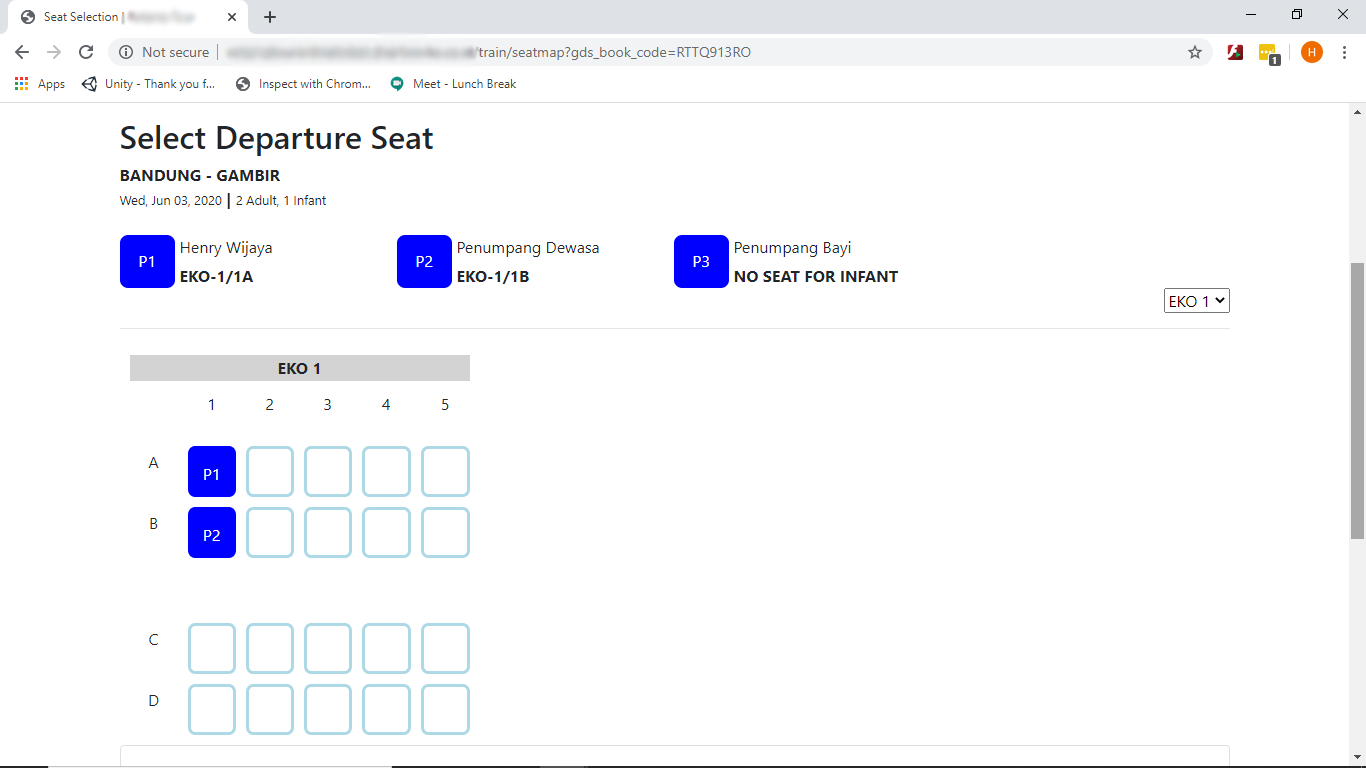
\includegraphics[width=\textwidth,height=\textheight,keepaspectratio]{Gambar/Seat Selection Depart.png}
        \caption{Hasil Pemilihan Kursi untuk Keberangkatan.}
            \label{img:pilihkursiberangkat}
        \end{figure}
        
        \begin{figure}[H]
        \center
        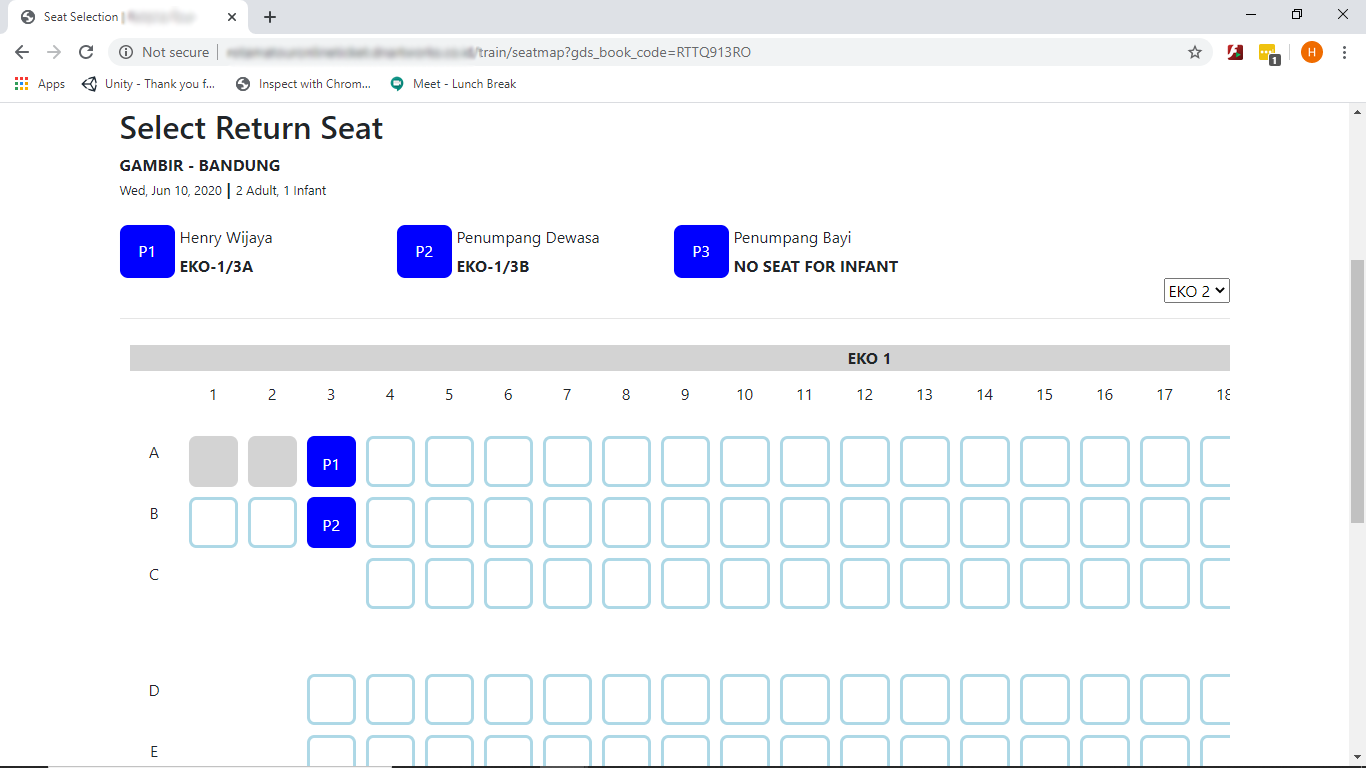
\includegraphics[width=\textwidth,height=\textheight,keepaspectratio]{Gambar/Seat Selection Return.png}
        \caption{Hasil Pemilihan Kursi untuk Pulang.}
            \label{img:pilihkursipulang}
        \end{figure}
        
        \item Menguji tombol \textit{back}.
        
        Tombol \textit{back} adalah tombol untuk kembali ke pilihan kursi berangkat jika pengguna sudah menekan tombol \textit{next train}. Sama dengan tombol \textit{next train}, tombol ini baru muncul jika pengguna memilih perjalanan pulang pergi. Tombol ini tidak mengembalikan kondisi pilihan kursi ke awal karena adanya tombol \textit{restore default}. Setelah dicoba, tombol ini berjalan dengan benar.
        
        \item Menguji tombol \textit{next}.
        
        Tombol \textit{next} di sini adalah tombol yang akan mengarahkan pengguna ke halaman konfirmasi. Saat tombol ditekan pengguna akan diberikan \textit{pop-up} untuk konfirmasi berisikan pilihan baru kursi penumpang seperti pada gambar \ref{img:konfirmasikursi}. Tombol ini berhasil memunculkan \textit{pop-up} yang menampilkan kursi yang dipilih pengguna. Saat pengguna sudah mengkonfirmasi pilihannya, tombol berhasil mengarahkan pengguna ke halaman konfirmasi dan pembayaran yang berarti tombol berjalan sesuai harapan.
        
        \begin{figure}[H]
        \center
        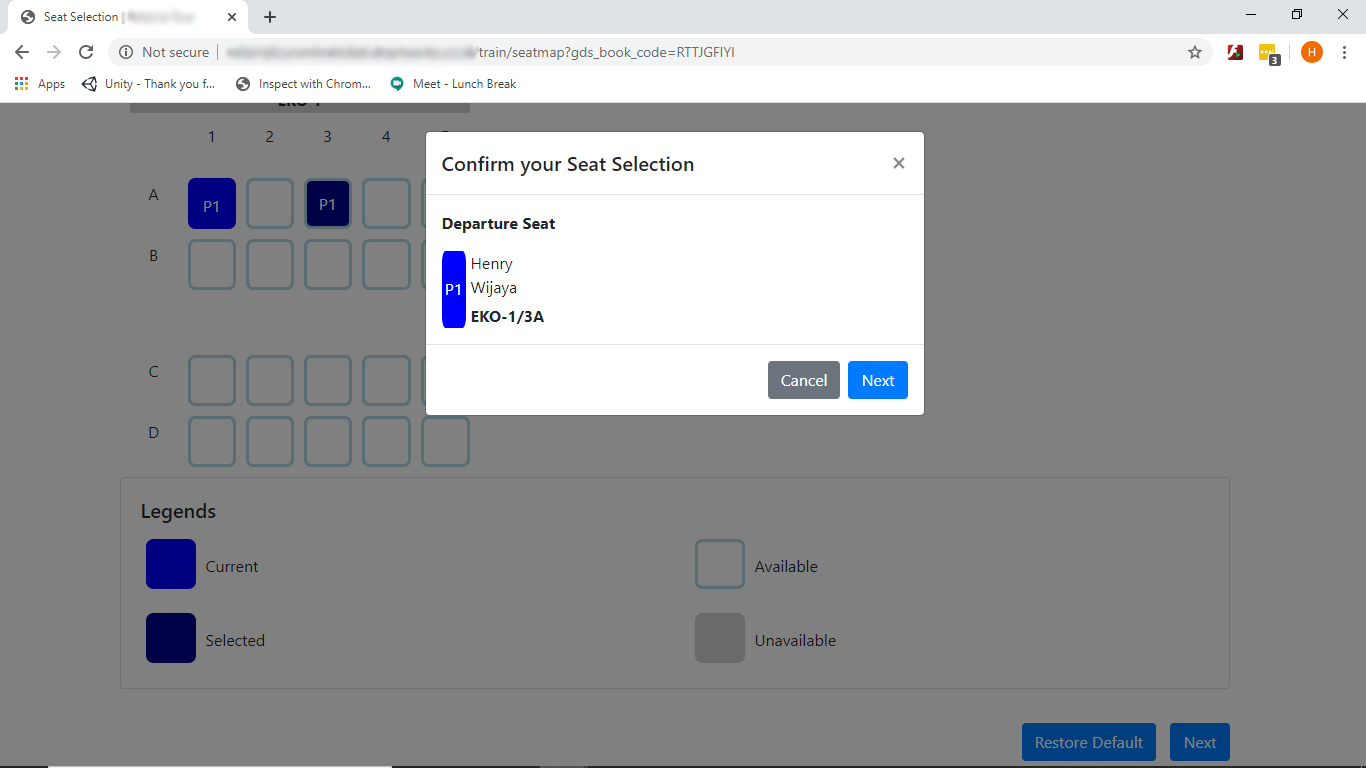
\includegraphics[width=\textwidth,height=\textheight,keepaspectratio]{Gambar/Konfirmasi pilih kursi.png}
        \caption{\textit{Pop-up} Konfirmasi Pemilihan Kursi.}
            \label{img:konfirmasikursi}
        \end{figure}
        
    \end{enumerate}
    
\subsection{Pengujian Halaman Konfirmasi dan Pembayaran.}
\label{subsec:pengujiankonfirmasi}

Halaman konfirmasi dan pembayaran belum diuji karena keterbatasannya waktu. Selain itu, belum ada kejelasan apakah \textit{API} yang digunakan akan menarik uang atau tidak. Pengujian yang sudah dilakukan di sini hanyalah sebatas pengujian tampilan awal dan masuk ke halaman pembayaran. Karena halaman ini menggunakan \textit{model} dan \textit{controller} Midtrans yang sudah diimplementasikan juga pada penerbangan, asumsi sementara adalah jika pengguna bisa masuk ke halaman pembayaran, maka halaman pembayaran berjalan dengan lancar.

\section{Analisis Hasil Pengujian}
\label{sec:analisishasiluji} 

Dari pengujian-pengujian yang sudah dilakukan, hampir semua fitur sudah dites dan berjalan dengan seharusnya. Pada saat pengujian, ada beberapa kasus yang menyebabkan hasil yang keluar tidak sesuai harapan. Kasus yang dimaksud adalah seperti saat mengisi data penumpang. Hal ini terjadi karena dokumentasi pada \textit{API} berbeda dengan respon yang diberikan pada saat modul tersebut diimplementasikan. 

Dokumentasi \textit{API} GDS menyebutkan penumpang bayi tidak perlu mengisi identitas. Pada kenyataannya saat membangun halaman ini, terjadi eror saat melakukan \textit{request} ke \textit{API}. Eror muncul karena \textit{API} mewajibkan identitas dari penumpang bayi dengan bentuk spesifik. Kadang saat pengujian, identitas bayi bisa masuk begitu saja saat memiliki alfabet tapi membutuhkan 16 karakter saat memasukkan angka saja. Dibutuhkan lebih banyak pengetesan dan kejelasan \textit{API} untuk menghindari eror yang tidak diinginkan.

Di luar API, pengujian fitur berjalan dengan lancar. Semua tombol dan fitur yang dibuat berjalan sesuai rancangan. Pengujian dilakukan setiap halaman selesai dibuat saat \textit{review} oleh rekan kantor. Sejauh ini belum ditemukan kejanggalan dalam pengetesan.